%% ISPRS Journal of Photogrammetry and Remote Sensing version of the benchmark
%% paper, generated from paper/manuscript.md by scripts/paper_to_elsevier.py.
%% Compile with pdfLaTeX and BibTeX (Overleaf's default). Search for TODO.
\documentclass[preprint,12pt,authoryear,a4paper]{elsarticle}
\usepackage[T1]{fontenc}
\usepackage{mathptmx}
% Courier and Helvetica, so no text font falls back to bitmap Computer Modern.
\renewcommand{\ttdefault}{pcr}
\renewcommand{\sfdefault}{phv}
\usepackage[a4paper,margin=2.5cm]{geometry}
\usepackage{amsmath}
\usepackage{graphicx}
% pdfTeX warns when a page holds several PDF figures that each carry a page
% group, as cairo writes them; the warning is harmless. Other engines skip this.
\ifdefined\pdfsuppresswarningpagegroup\pdfsuppresswarningpagegroup=1\relax\fi
\usepackage{array}
\usepackage{tabularx}
\usepackage{booktabs}
% Landscape pages for the tables too wide for the portrait text width.
\usepackage{rotating}
\usepackage{url}
\urlstyle{same}
\usepackage[hidelinks]{hyperref}
\usepackage{lineno}
\providecommand{\tightlist}{\setlength{\itemsep}{0pt}\setlength{\parskip}{0pt}}
\newcolumntype{L}{>{\raggedright\arraybackslash}X}
\newcolumntype{R}{>{\raggedleft\arraybackslash}X}
\newcolumntype{C}{>{\centering\arraybackslash}X}
\graphicspath{{./}{../}}
\setlength{\emergencystretch}{2em}
% DOIs as https://doi.org/ links and URLs without a label, as the journal's
% reference style prints them; elsarticle-harv.bst defines these only when
% they are undefined.
\newcommand{\DOIprefix}{}
\newcommand{\URLprefix}{}
\newcommand{\doi}[1]{\url{https://doi.org/#1}}

% The journal lists a group of citations alphabetically, then chronologically,
% as the reference list is sorted. elsarticle passes this option to natbib on
% the next run.
\biboptions{sort}
\journal{ISPRS Journal of Photogrammetry and Remote Sensing}

\begin{document}

\begin{frontmatter}

\title{Choosing tree detectors by point density: a field-stem benchmark for national-mapping airborne LiDAR}

% TODO: complete the author block: every author, each affiliation with its full
% postal address and country, and the corresponding author's e-mail address.
\author[aff1]{Alexey Grigoryev\corref{cor1}\fnref{orcid1}}
\cortext[cor1]{Corresponding author.}
\fntext[orcid1]{ORCID: \url{https://orcid.org/0009-0008-1571-4774}.}
\ead{TODO}
\affiliation[aff1]{organization={TODO},
            city={TODO},
            country={TODO}}

\begin{abstract}
Deep 3D tree segmenters are developed on dense laser scans, while national
mapping programmes deliver airborne laser scanning at a few pulses per square
metre. We scored three published learned 3D detectors, zero-shot, six classical
and two aerial-image detectors against 2,525 field-mapped stems in 106 plots at
five National Ecological Observatory Network sites in California and Washington,
at native density (median 9.8 pulses/m\textsuperscript{2}) and five thinned densities down to 0.6
pulses/m\textsuperscript{2}. At native density and a 4 m match radius, ForestFormer3D and
SegmentAnyTree lead a canopy-height-model baseline by 0.048 and 0.044 F1, but
randomly shifted detections reach 70--79\% of every detector's F1. In
chance-corrected F1 SegmentAnyTree leads by 0.03 on nominal plot cores and by
0.06 inside censused subplots; in Washington, the held-out region, the
nominal-core lead does not exclude zero and the censused lead does so narrowly,
and not in sensitivity checks. ForestFormer3D's lead of 0.02--0.03 does not
exclude zero. SegmentAnyTree holds down to 1.8 pulses/m\textsuperscript{2} and
collapses below it, just under the U.S. Geological Survey quality level 2 floor
of 2 pulses/m\textsuperscript{2}, while ForestFormer3D and TreeisoNet degrade gracefully;
native-density rank predicts rank down to 1.8 pulses/m\textsuperscript{2} (Spearman 0.71), not
below it ($-$0.05). Below native density the five-site leads over the baseline
rest on its smoothing rule. For users, ForestFormer3D run at every density does
as well in Washington as a post hoc rule, selected on California, that runs
SegmentAnyTree from 2 pulses/m\textsuperscript{2} up and a canopy-model detector below. Clips,
detections and code are public.
\end{abstract}

\begin{highlights}
\item Eleven tree detectors scored against 2,525 field stems; eight at six densities.
\item Shifted copies reach 70--79\% of native F1 at 4 m; above them one segmenter leads.
\item Its lead is 0.03 on nominal plot cores and 0.06 inside censused subplots.
\item SegmentAnyTree collapses below 1.8 pulses/m\textsuperscript{2}; ForestFormer3D and TreeisoNet do not.
\item Native-density rank predicts rank down to 1.8 pulses/m\textsuperscript{2}, not below it.
\end{highlights}

\begin{keyword}
individual tree detection \sep airborne laser scanning \sep point density \sep deep learning \sep instance segmentation \sep chance agreement
\end{keyword}

\end{frontmatter}

\linenumbers

\section{Introduction}\label{sec:1}

Individual tree detection from airborne laser scanning (ALS) feeds forest
inventory, carbon accounting, fuel mapping and habitat models. The data that
most practitioners can obtain for a whole ownership or a whole state come from
national mapping programmes. The U.S. Geological Survey (USGS) 3D Elevation
Program (3DEP) specifies an aggregate nominal pulse density of at least 2
pulses/m\textsuperscript{2} for quality level 2 (QL2) and at least 8 pulses/m\textsuperscript{2} for quality level 1
(QL1) \citep{usgs2026topographic}. These are the densities at which national
programmes deliver data wall to wall.

Two literatures have grown around the task, and they rarely meet. Classical
detectors were developed and compared on conventional airborne scans of about 1
to 25 pulses/m\textsuperscript{2} \citep{kaartinen2012international,jakubowski2013tradeoffs,sparks2022crosscomparison}. They include local maxima on a canopy height model
(CHM) with a height-dependent window \citep{popescu2004seeing}, region growing in the
point cloud \citep{li2012new}, multi-scale point segmentation \citep{vega2014ptrees} and
adaptive mean shift \citep{ferraz2016lidar}. Deep 3D instance segmenters
\citep{wielgosz2024segmentanytree,xiang2025forestformer3d,xi2025new} are trained
mostly on unmanned, mobile and terrestrial laser scanning. They are benchmarked
on those scans and on high-density airborne scans, at hundreds to thousands of
points per square metre \citep{puliti2023forinstance,ruoppa2026benchmarking}.

Whether the published checkpoints of these segmenters help at national-mapping
density is therefore open, and four obstacles stand in the way of answering it.
First, we found no per-point instance labels at such densities (Section~\ref{sec:2.1}), so
the reference has to be field-mapped stems, which are incomplete: a detection of
a real but unmapped tree counts as an error. Second, sparse acquisitions are
usually simulated by thinning a dense one, as in \citet{jakubowski2013tradeoffs}, and
the simulation is rarely checked against a native sparse flight of the same
stand. Third, research code has to be adapted to new data, and an adapter defect
can be mistaken for domain shift. Fourth, a match radius wide enough to absorb
stem-mapping error also admits coincidental matches, whose share stem benchmarks
do not report.

We address the question with a benchmark built to control those obstacles, and
ask four research questions:

\begin{itemize}
\tightlist
\item
  RQ1. At QL1 density, do published zero-shot 3D segmenters detect field-mapped
  stems better than a density-aware canopy-model baseline, beyond what chance
  co-location explains?
\item
  RQ2. How does each detector degrade toward and below the QL2 floor?
\item
  RQ3. Does a detector's rank at native density predict its rank on sparser
  clouds?
\item
  RQ4. Which detector should a user of national-mapping LiDAR run at each USGS
  quality level, given a GPU or only a CPU?
\end{itemize}

Our contributions are:

\begin{enumerate}
\tightlist
\item
  A field-stem benchmark of eleven detectors (three zero-shot learned, six
  classical, two RGB) at five National Ecological Observatory Network (NEON)
  sites in two regions, on fixed evaluation clips at six densities from 9.8 to
  0.6 pulses/m\textsuperscript{2}, with paired plot-bootstrap intervals.
\item
  An evaluation protocol that makes such scores comparable: chance-corrected
  scores from a shift null, on nominal plot cores and inside censused subplots,
  with a simulation of the correction; precision bracketed by censused subplots
  and a co-detection credit; decimation checked against native sparse flights;
  and a dense-domain positive control.
\item
  An open harness whose tables rebuild with one command.
\end{enumerate}

RQ4 is answered as guidance in the discussion (Section~\ref{sec:6.1}), with a decision
table by measured density and compute budget that was designed after the
five-site results were known (Section~S25).

\section{Related work}\label{sec:2}

\subsection{Benchmarks and point density}\label{sec:2.1}

Open benchmarks with per-point tree labels are dense: about 500 to 9,500
points/m\textsuperscript{2} in the FOR-instance collections \citep{puliti2023forinstance} and more than
1,000 points/m\textsuperscript{2} in the helicopter ALS of FGI-EMIT \citep{ruoppa2026benchmarking}.
FOR-instance v3 spans 10 to 50,000 points/m\textsuperscript{2} without stating how its sparsest
clouds were obtained \citep{wielgosz2026segmentanytreev2}. NeonTreeEvaluation
\citep{weinstein2021benchmark} and the IDTReeS competitions \citep{marconi2019data,graves2023data} are built on NEON's airborne data, its sparse ALS included, but
annotate crowns in imagery or the field and use stems for recall or crown
correspondence, not for precision. International comparisons scored classical
detectors against field stems on conventional airborne scans
\citep{kaartinen2012international,vauhkonen2012comparative,eysn2015benchmark,wang2016international}. We found no published benchmark that scores deep 3D
segmenters against field stems at national-mapping density.

Density studies follow the same split. Classical work varies density from below
1 to about 25 pulses/m\textsuperscript{2} \citep{hirata2004effects,jakubowski2013tradeoffs,kaartinen2012international,sparks2022crosscomparison}. \citet{hirata2004effects}
found that tree-top extraction from a canopy model declined suddenly below 3 to
5 points/m\textsuperscript{2} in first-pulse data thinned from a denser flight, and
\citet{sparks2022crosscomparison} compared classical detectors on two ALS datasets of
the same stands, at 8 and 22 pulses/m\textsuperscript{2}, without testing decimation. Deep-model
studies subsample dense scans to between 10 and 1,000 points/m\textsuperscript{2}
\citep{wielgosz2024segmentanytree,xiang2025forestformer3d}. On FGI-EMIT subsampled
to 10 points/m\textsuperscript{2}, a retrained ForestFormer3D and the published SegmentAnyTree
keep a roughly stable F1 \citep{ruoppa2026benchmarking}. \citet{yu2004effects} flew one
boreal area at about 10, 5 and 2.5 points/m\textsuperscript{2} and thinned the densest data to the
sparser two. Thinned and native data found as many trees at 5 points/m\textsuperscript{2} (1,416
against 1,400) but not at 2.5 (1,331 against 532). The authors attribute that
loss to missing canopy returns at altitude rather than to density alone; we read
it as thinning being strongly optimistic. The nearest evaluation of a pretrained
segmenter on conventional ALS is that of \citet{destouches2026weaklysupervised}, who
ran the published SegmentAnyTree on Swiss aircraft ALS at 38 points/m\textsuperscript{2}. They
counted instances on four 1 ha tiles labelled by hand and completed with
visually validated automatic detections. Recall by crown class, canopy layer or
height class has been reported for classical methods \citep{wang2016international,hamraz2017forest,cao2023benchmarking}, one of them designed for layered
canopies \citep{hamraz2017forest}.

The nearest concurrent work is a public repository of code and results without a
paper, whose only commit dates from November 2026
\citep{mallacampoverde2026pretrained}. It scores the released SegmentAnyTree,
ForestFormer3D and TreeLite3D \citep{rizaldy2026labelefficient} weights and two
classical methods against a field inventory of 1,437 trees on 22 alpine ALS
plots, by crown stratum, and thins the denser site by pulse from about 120 to
about 30 points/m\textsuperscript{2}. That is still an order of magnitude denser than
national-mapping data.

We found no published study that evaluates a pretrained 3D segmenter on native
ALS at 1 to 2 pulses/m\textsuperscript{2}. We found none that checks decimation against a native
sparse acquisition for a detector's precision and recall against field stems or
with learned detectors. We found no report of understory recall for a deep model
below 20 points/m\textsuperscript{2}.

\subsection{Evaluation conventions}\label{sec:2.2}

Dense-cloud benchmarks match instances one to one at an intersection over union
(IoU) of 0.5 \citep{puliti2023forinstance,xiang2025forestformer3d,ruoppa2026benchmarking}. Stem benchmarks use restricted nearest neighbours
\citep{eysn2015benchmark}, optimal assignment \citep{hamraz2016robust,kuhn1955hungarian}
or integer programming \citep{hershey2022voxelbased}, and one-to-one matching within
4 m has linked image detections to national-inventory trees
\citep{gominski2025mining}. We found no published forestry study that scores the same
detections under greedy and optimal assignment and across radii, or that reports
the score that randomly shifted copies of the same detections would reach; the
concurrent repository of Section~\ref{sec:2.1} compares greedy with optimal matching and
reports the score of uniformly placed detections. The devices exist elsewhere:
the toroidal shift is the independence null of spatial point-pattern analysis
\citep{lotwick1982methods,wiegand2004rings}, forecast verification corrects threat
scores for hits expected by chance \citep{hogan2010equitability}, and F1 itself
carries no chance level \citep{powers2011evaluation}. Reference incompleteness is
seldom measured, although \citet{hershey2022voxelbased} found most raw false positives
to be trees below the recording threshold or missed by the crew. Double-observer
surveys estimate what one observer misses \citep{nichols2000doubleobserver}; we found
no tree benchmark that brackets precision this way. Leakage audits and
reproducibility standards are established in machine learning
\citep{kapoor2023leakage,heil2021reproducibility}, as is reporting the stability of
a ranking with intervals \citep{dehghani2021benchmark,agarwal2021deep}. We found no
audit of overlap between a checkpoint's training data and a benchmark's test
data, and no forestry detector benchmark that reports the stability of its
ranking.

\subsection{Recent models}\label{sec:2.3}

Newer models, SegmentAnyTreeV2 \citep{wielgosz2026segmentanytreev2}, SelectAnyTree
\citep{nguyen2026selectanytree}, ForestMamba \citep{nguyen2026forestmamba}, ForPT
\citep{yue2026toward}, ITS-Net \citep{li2026itsnet} and ForestQuery
\citep{zhan2026forestquery}, report no performance at 1 to 8 pulses/m\textsuperscript{2}, and of these
only ForestMamba has public instance-segmentation weights. These statements,
like the statements of absence in Sections~\ref{sec:2.1} and \ref{sec:2.2}, rest on a scan of about
ninety primary sources completed on 30 September 2026 and on literature and
repository checks completed on 21 October 2026 and repeated on 16 November 2026
(Section~S24). We therefore evaluate the first SegmentAnyTree
\citep{wielgosz2024segmentanytree}, ForestFormer3D \citep{xiang2025forestformer3d} and
TreeisoNet \citep{xi2025new}. ForestMamba, run after the tables were fixed, is
reported in Section~S23. Two further models with public weights, TreeLite3D
\citep{rizaldy2026labelefficient} and ForestSeg3D \citep{zhang2026forestseg3d}, came to
our notice in November 2026, after the runs, and are not evaluated.

\section{Data}\label{sec:3}

\subsection{Sites and airborne LiDAR}\label{sec:3.1}

The benchmark uses five terrestrial NEON sites in two regions (Table~\ref{tab:1}, Fig.~\ref{fig:1}).
San Joaquin Experimental Range (SJER), Soaproot Saddle (SOAP) and Lower
Teakettle (TEAK) lie on a gradient of canopy closure in the Sierra Nevada of
California. Wind River Experimental Forest (WREF), an old-growth forest, and
Abby Road (ABBY), a young, even-aged managed stand, are Douglas-fir forests in
Washington. All were flown by the NEON Airborne Observation Platform in 2021
\citep{neon2026discrete}. Inside the benchmark plot cores the discrete-return clouds
have a median density of 18.7 points/m\textsuperscript{2} and 9.8 first-return pulses/m\textsuperscript{2}, close to
the QL1 specification. The stands differ in density and size as much as in type
(Table~S14).

\begin{table}[!htbp]
\centering
{\scriptsize
\setlength{\tabcolsep}{3pt}
\renewcommand{\arraystretch}{1.15}
\begin{tabularx}{\linewidth}{l>{\hsize=1.86998\hsize\linewidth=\hsize}L>{\hsize=1.25\hsize\linewidth=\hsize}L>{\hsize=0.61\hsize\linewidth=\hsize}Lr>{\hsize=0.77\hsize\linewidth=\hsize}L>{\hsize=0.88\hsize\linewidth=\hsize}L>{\hsize=0.62\hsize\linewidth=\hsize}L}
\toprule
Site & Forest & 2021 flight & Plots & Stems & Crown classes & Pulses/m\textsuperscript{2} & Censused plots / references \\
\midrule
SJER & Open oak and foothill pine woodland, California & 31 March, RIEGL Q780 & 6 (6 / 0) & 57 & 27 / 1 / 29 & 10.5 (5.4--15.8) & 2 / 14 \\
SOAP & Mixed conifer, California & 12--13 July, Galaxy Prime & 18 (7 / 11) & 231 & 184 / 44 / 3 & 12.2 (7.4--18.7) & 1 / 2 \\
TEAK & Red fir and subalpine conifer, California & 13--14 July, Galaxy Prime & 19 (6 / 13) & 374 & 316 / 52 / 6 & 10.2 (7.1--22.5) & 9 / 119 \\
WREF & Old-growth Douglas-fir and western hemlock, Washington & 18--24 July, Galaxy Prime & 38 (20 / 18) & 1,063 & 638 / 404 / 21 & 8.7 (5.0--19.9) & 28 / 642 \\
ABBY & Managed Douglas-fir, Washington & 19 and 24 July, Galaxy Prime & 25 (13 / 12) & 800 & 707 / 91 / 2 & 10.0 (5.9--16.2) & 17 / 413 \\
All &  &  & 106 (52 / 54) & 2,525 & 1,872 / 592 / 61 & 9.8 (5.0--22.5) & 57 / 1,190 \\
\bottomrule
\end{tabularx}
}
\caption{Sites and reference population. Plots are tower / distributed.
Crown classes are overstory (dominant and codominant) / understory (intermediate
and suppressed) / not classed. Pulse density is the median and range of
first-return density inside the plot cores at native density.}
\label{tab:1}
\end{table}

\begin{figure}[!htbp]
\centering
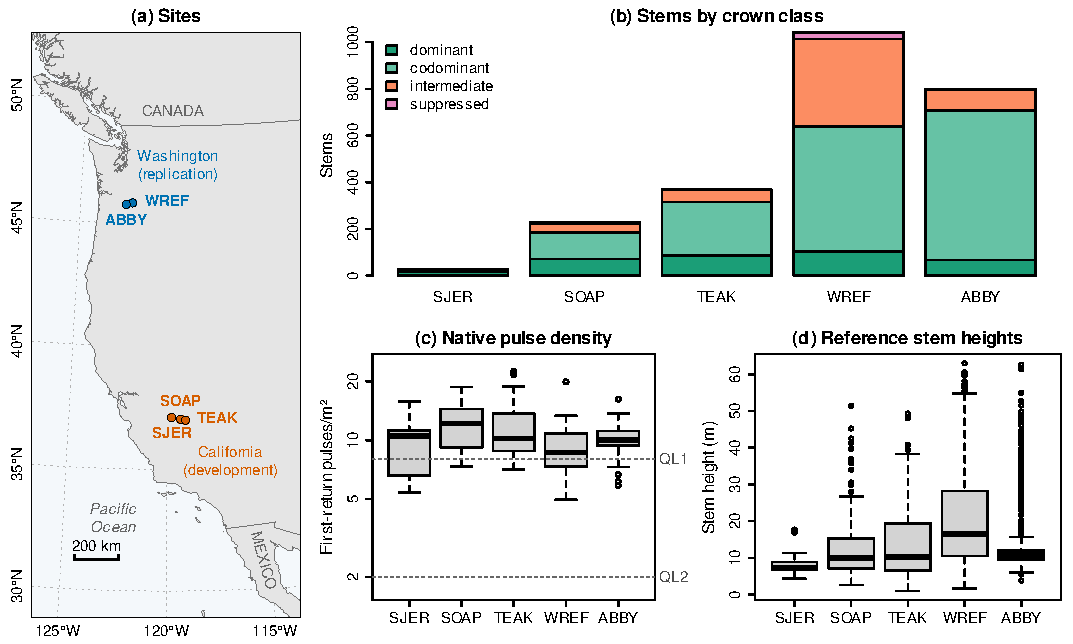
\includegraphics[width=\textwidth]{figures/figure_1.pdf}
\caption{Sites and reference population. (a) The five NEON sites: SJER,
SOAP and TEAK in California, the development region, and WREF and ABBY in
Washington, the replication region; each point is the mean position of the
site's plots. Albers equal-area projection; base map from Natural Earth (public
domain). (b) Classed stems by field crown class at each site; the 61 stems
without a crown class, 29 of them at SJER, are not shown. (c) First-return pulse
density inside the plot cores at native density; the dotted lines mark the QL1
(8 pulses/m\textsuperscript{2}) and QL2 (2 pulses/m\textsuperscript{2}) floors. (d) Field heights of the reference
stems.}
\label{fig:1}
\end{figure}

\subsection{Field reference}\label{sec:3.2}

The reference is the NEON woody vegetation structure product, in its
RELEASE-2026 \citep{neon2026vegetation}. Each mapped stem is located from its
recorded distance and azimuth to a surveyed point of its plot, with the
coordinates and uncertainties of the NEON location service, and paired with its
measurement nearest to 2021 within four years, which supplies its status,
height, diameter at breast height (DBH) and canopy position. A stem is one bole
record: a multi-stemmed tree contributes each of its boles that passes the rules
below, and 37 records are additional boles of 20 trees, 27 of them at SJER
(Section~S14). The population was declared before the runs reported here and
before any detector was run on the Washington sites; its six-tree rule dates
from the earlier development phase of Section~\ref{sec:4.5}, and its DBH floor was set
from the Washington field data without detector scores.

A reference stem is live, mapped, at least 10 cm in DBH and inside the nominal
plot core: the 40 m $\times$ 40 m of a tower plot or the central 20 m $\times$ 20 m of a
distributed plot. A plot enters if it holds at least six live mapped trees of at
least 10 cm DBH over the whole plot, which gives 106 plots and 2,525 stems.
Crown classes follow NEON's canopy position (Table~\ref{tab:1}): open-grown and full-sun
crowns are dominant, partially shaded crowns codominant, mostly shaded crowns
intermediate and fully shaded crowns suppressed. Two ABBY stems without a canopy
position are classed by their height rank within the plot; 61 stems have no
class and count only in the totals. Of the 592 understory stems 404 are at WREF,
so understory results mostly describe that old-growth site. At SOAP a wildfire
may have passed between part of the reference and the flight: the perimeter of
the 2020 Creek Fire as CAL FIRE maps it contains six of the 18 plots, while the
interagency copy of the same perimeter, about 0.9 km away, contains none, and a
perimeter does not give burn severity. The three distributed plots among the six
(22 stems) were last measured in 2019, and all eleven distributed plots at SOAP
(96 stems) before the fire. Leaving the three out moves no five-site corrected
lead at 4 m by more than 0.002 (Section~S14).

\subsection{Evaluation clips and density levels}\label{sec:3.3}

For each plot we clip the core plus a 25 m buffer from the tiles, normalise
heights with a triangulated ground surface, and store the raw and normalised
clips and a 1 m terrain model. These fixed evaluation clips are hashed (SHA-256
of every file), so that every detector reads identical bytes, and are
reproducible byte for byte. Sparser acquisitions are simulated by thinning
(decimating) all returns to a target density on a 5 m grid, with a seed derived
from the site, plot and target, before normalisation, so that the terrain model
also sees the sparser cloud. The density series has all-return targets of 8, 4,
2 and 1 points/m\textsuperscript{2} and one of 3.2 points/m\textsuperscript{2}, declared before any detector was run
on it and chosen from measured densities alone so that its median over the whole
clips is 2.0 pulses/m\textsuperscript{2}, the QL2 floor; this QL2 level was cut as a separate set
of clips with the same population and seed rule.

We report first-return density, the quantity that specifications state, inside
the plot core, the area that is scored: a median of 9.8 pulses/m\textsuperscript{2} at native
density and 4.4, 2.2, 1.8, 1.1 and 0.6 pulses/m\textsuperscript{2} on the five thinned levels
(Section~S26). Whole-clip densities are about 10\% higher on the thinned levels
(4.7, 2.5, 2.0, 1.3 and 0.6 pulses/m\textsuperscript{2}), because the thinning grid is not aligned
with the clip and its partial edge cells keep proportionally more returns. The
QL2 level, declared on the whole-clip figure, therefore sits at 1.8 pulses/m\textsuperscript{2} in
the cores, with 79 of its 106 cores below 2 pulses/m\textsuperscript{2}. The baseline's density
rules (Section~\ref{sec:4.1}) read the whole-clip density, as in the runs. Thinning
removes returns rather than whole pulses and equalises density across the 5 m
cells, so the thinned levels lack the swath-overlap and scan-angle variation of
a real acquisition. Each level is one seeded realisation shared by all
detectors. At the three California sites, on an earlier population without the
DBH floor, eleven independent seeds give a standard deviation of per-site F1 of
0.005 to 0.028 for the baseline; the spread was not measured for the other
detectors.

\subsection{Native sparse flights and 3DEP clouds}\label{sec:3.4}

To test thinning we use earlier NEON flights of the same plots that are natively
sparse: SJER in March 2017 and SOAP and TEAK in June 2018, flown in NEON's
Optech Gemini era, with median first-return densities in the plot cores of 3.1,
4.1 and 5.0 pulses/m\textsuperscript{2} at SJER, TEAK and SOAP; references were rebuilt for those
years. A cross-sensor check uses public USGS 3DEP clouds over the 43 California
plots \citep{usgs2026usgs}, extracted with PDAL \citep{butler2021pdal} and used without
the points that the surveys classify as noise or flag as withheld, about 5\% of
the points at SOAP and TEAK. None of the covering surveys is at QL2 density
(medians of 41, 28 and 5.5 pulses/m\textsuperscript{2} in the plot cores at SOAP, TEAK and SJER),
so the check compares 3DEP and NEON clouds thinned to the same target.

\subsection{Dense-domain control data}\label{sec:3.5}

FGI-EMIT \citep{ruoppa2026benchmarking,ruoppa2026fgiemit} provides manual per-point
tree labels for 1,561 trees in 19 plots of boreal forest in Espoo, Finland,
scanned from a helicopter at more than 1,000 points/m\textsuperscript{2}. Its six test plots had
been scored in a first transfer experiment and two training plots used in the
adapter audit of Section~\ref{sec:5.7}, so before running any model on the other eleven
training plots we set three aside as an untouched reserve (257 trees) by a rule
on published stand density. The remaining eight and the two audit plots form the
development set (841 trees), on which the detector policy was selected before
the reserve was evaluated once. Points of trees that the release leaves
unlabelled as partial (about 4\% of the points) are removed, so every tree left
is a reference tree, a cleaner scene than any survey would give. We found no
documented overlap between the published training lists of both checkpoints and
FGI-EMIT, but no source gives a complete training history of the released
weights, so the reserve is a within-dataset check, not an independent test.

\section{Methods}\label{sec:4}

Fig.~\ref{fig:2} outlines the evaluation protocol.

\begin{figure}[!htbp]
\centering
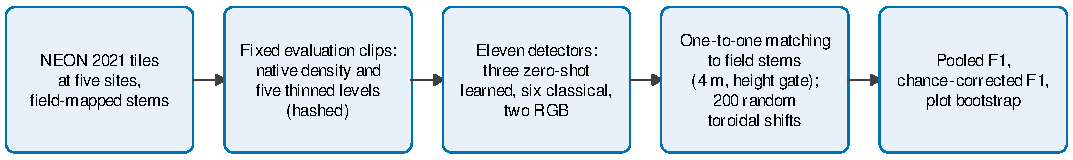
\includegraphics[width=\textwidth]{figures/figure_2.pdf}
\caption{The evaluation protocol. Fixed evaluation clips at native
density and five thinned density levels are cut from the NEON 2021 tiles and
hashed, so that every detector reads identical bytes; each detector's detections
are matched one to one to the field stems (greedy, within 4 m, with the height
gate) and scored against 200 random toroidal shifts of the same detections;
scores are pooled over plots, corrected for chance and given plot-bootstrap
intervals (Sections~\ref{sec:4.2} and \ref{sec:4.4}).}
\label{fig:2}
\end{figure}

\subsection{Detectors}\label{sec:4.1}

Table~\ref{tab:2} lists the detectors. ForestFormer3D, SegmentAnyTree and TreeisoNet are
published as instance segmenters; we reduce the instances of the first two to
their apexes and call them the segmenters, use TreeisoNet's localisation network
as a detector, and call all three the learned detectors.

\begin{table}[!htbp]
\centering
{\scriptsize
\setlength{\tabcolsep}{3pt}
\renewcommand{\arraystretch}{1.15}
\begin{tabularx}{\linewidth}{>{\hsize=0.87\hsize\linewidth=\hsize}L>{\hsize=1.44998\hsize\linewidth=\hsize}L>{\hsize=0.63\hsize\linewidth=\hsize}L>{\hsize=1.27\hsize\linewidth=\hsize}L>{\hsize=1.09\hsize\linewidth=\hsize}L>{\hsize=0.69\hsize\linewidth=\hsize}L}
\toprule
Detector & Type & Input & Training data & Implementation & Compute \\
\midrule
CHM-VWF & Local maxima on a canopy height model, height-dependent window \citep{popescu2004seeing} & Normalised cloud, first returns & None & lasR \citep{roussel2026lasr} & CPU, 2.9 s per plot \\
\texttt{multichm} & Local maxima over a stack of height-sliced canopy models, after \citet{eysn2015benchmark} & Normalised cloud & None & lidRplugins \citep{roussel2023lidrplugins}; density-derived resolution and CHM-VWF window & CPU, 6.0 s per plot \\
\texttt{lmfauto} & Point local maxima, automatic window & Normalised cloud & None & lidRplugins & CPU, 2.3 s per plot \\
\texttt{ptrees} & Multi-scale point segmentation \citep{vega2014ptrees} & Normalised cloud & None & lidRplugins & CPU, 3.2 s per plot \\
AMS3D & Adaptive mean shift in 3D \citep{ferraz2016lidar} & Normalised cloud & None & crownsegmentr \citep{steinmeier2025crownsegmentr} & CPU, 5.0 s per plot \\
Li 2012 & Point-cloud region growing \citep{li2012new} & Normalised cloud & None & lidR \citep{roussel2020lidr} & CPU, 3.7 s per plot \\
ForestFormer3D & Transformer instance segmentation \citep{xiang2025forestformer3d} & Raw cloud, whole scene & FOR-instanceV2: unmanned, mobile and terrestrial laser scanning \citep{xiang2025forinstancev2}; training density not stated & Published code and weights (Table~S15) & GPU, 97.9 s per plot; about 3.4 GPU-hours per km\textsuperscript{2} \\
SegmentAnyTree & Sparse convolutional instance segmentation \citep{wielgosz2024segmentanytree} & Raw cloud & FOR-instance unmanned scans and Norwegian mobile scans, with copies sparsified to 1,000, 500, 100, 75, 50, 25 and 10 points/m\textsuperscript{2} & Published code and weights (Table~S15) & GPU, 411.1 s per plot; about 14 GPU-hours per km\textsuperscript{2} \\
TreeisoNet & Tree localisation and offset networks \citep{xi2025new}; the airborne checkpoints distributed with TreeAIBox & Normalised cloud, 0.8 $\times$ 0.8 $\times$ 2.0 m voxels for tree tops & Unmanned laser scanning of reclaimed wellsites at about 1,160 points/m\textsuperscript{2}, the data described for TreeAIBox's wellsite models \citep{movchan2025uavbased}; the match to the files we ran is inferred from their names & TreeAIBox \citep{nrcan2025treeaibox} & GPU, 7.9 s per plot; about 16 GPU-minutes per km\textsuperscript{2} \\
DeepForest & Crown boxes in RGB imagery \citep{weinstein2020deepforest} & 10 cm camera mosaic \citep{neon2026camera} & Crowns from 22 NEON sites, then hand annotations from six, including SJER and TEAK & \texttt{deepforest-tree} \citep{weecology2024deepforesttree} & GPU, 265.7 s per site \\
Detectree2 & Crown polygons in RGB imagery \citep{ball2023accurate} & 10 cm camera mosaic & Tropical forests and an urban site & Published weights \citep{ball2025detectree2} & CPU, 8.1 s per plot \\
\bottomrule
\end{tabularx}
}
\caption{Detectors. The three learned point detectors are used zero-shot
with their published checkpoints. DeepForest's training annotations include two
of the benchmark sites, SJER and TEAK, so it is not zero-shot there. Compute:
device and median wall time per call at native density on nine plots, start-up,
clip reading and model loading included, on an Intel Core i9-14900K and one
NVIDIA RTX 5090 (DeepForest predicts a whole site at once), with the cost per
square kilometre scaled from the clip area, before tiling overhead (Section~S22); the classical detectors cost a few CPU-minutes per km\textsuperscript{2}.}
\label{tab:2}
\end{table}

\textbf{The baseline.} CHM-VWF, local maxima on a canopy height model found with a
variable window filter, derives its parameters from measured density. Its canopy
model is a triangulation of first returns, rasterised at 0.25 m when the clip
has 8 pulses/m\textsuperscript{2} or more and at 0.5 m below that, with pits filled by lasR's fill
of the rasterised surface, not by the pit-free algorithm of
\citet{khosravipour2014generating}. Below 8 pulses/m\textsuperscript{2}, as on 18 of the 106 plots at
native density, the surface is smoothed with a circular moving mean 3 m across.
This smoothing, the baseline's pre-declared smoothing rule, is a rule of thumb
fixed before the runs; a run without it was added post hoc (Section~\ref{sec:5.2}). Tree
tops are local maxima above 2 m in a circular window of diameter 0.1 h + 3 m,
clamped to 3 to 5 m.

\textbf{Other detectors.} \texttt{multichm} shares the baseline's density-derived resolution
and window, without smoothing (Table~\ref{tab:2}). The other classical detectors use
package defaults or fixed parameters not adapted to density: \texttt{ptrees} takes the
package's example neighbourhoods of 30 and 15 points, and AMS3D crown diameter-
and length-to-height ratios of 0.4 and 0.8, which the configuration record
(Section~S11) attributes to \citet{ferraz2016lidar}. Li 2012 runs at native density
only. The learned detectors run with the inference settings of the published
code and checkpoints (Table~S15), ForestFormer3D on whole scenes (Section~\ref{sec:5.7});
no detector removes the few points that NEON classifies as noise (Section~S15).
Their apexes have no 2 m height floor, unlike the classical detectors'; applying
it would raise ForestFormer3D's F1 by at most 0.013 if every apex below 2 m is a
false positive (Section~S18). TreeisoNet's confidence threshold of 0.22 was
chosen by hand on five SOAP plots at the checkpoint's own voxel, in a selection
that was not scripted and whose plots were not recorded, and was not
recalibrated for the coarser airborne voxel used here; at a fixed threshold the
two voxels give detection counts that differ by up to half. RGB crowns become
detections at their box centres or polygon centroids, with the height of a 0.5 m
highest-return raster of the plot's native clip at that point, or 2 m where that
raster is empty. SAM2Point \citep{guo2024sam2point}, prompted with CHM-VWF tops, is
reported in Sections~S10 and S21 but not analysed.

\subsection{Scoring and chance agreement}\label{sec:4.2}

Reference stems in the plot core are matched one to one to detections in the
core or within 4 m of it, greedily by increasing horizontal distance. A height
gate keeps a short stem from taking a tall neighbour's apex: a detection's
height must lie between half the stem's height and that height plus 8 m, and
stems without a height are matched on position alone. The 4 m radius covers the
stem-mapping uncertainty and the offset between stem base and crown apex; it is
eight to ten times the recorded stem uncertainty and follows one-to-one matching
within 4 m of field-inventory trees \citep{gominski2025mining}. Native-density
accuracy, the density response, rank stability, the regional contrast and
understory recall are also given at 2 m (Table~\ref{tab:3}, Section~\ref{sec:5.4}, Sections~S12 and
S21); the censused precision, the native-flight comparison, the dense-domain
control and the decision table of Section~S25 are scored at 4 m only, and the
chance null inside censused subplots also at 2 m (Section~S12). Recall is the
share of reference stems matched and precision the share of core detections
matched, F1 their harmonic mean, and rates are pooled by summing counts over the
plots that every detector scored, never by averaging plot rates.

\textbf{Chance agreement.} The plot cores hold 1.2 reference stems per 4 m circle,
and the detectors place 0.6 to 4.7 core detections per reference stem, so part
of every match is co-location. We measure it with a random toroidal shift
\citep{lotwick1982methods,wiegand2004rings}: in each plot the detections in the
core and its matching margin are shifted together by a random offset of at
least 8 m and wrapped at the edges of that square, which keeps their number
and heights, and their relative positions except across the wrapped edge. The
same 200 offsets serve every detector and density, and a detector's null F1 is
computed from its mean counts over the shifts (Section~S12). If a share s of
stems is found by skill and the rest only by chance, recall = s + (1 $-$ s) $\times$
null. By the same reasoning, as Cohen's kappa corrects agreement for chance
\citep{cohen1960coefficient}, we report corrected F1,
\begin{equation}
F_1^{\mathrm{c}} = \frac{F_1 - F_1^{0}}{1 - F_1^{0}}
\end{equation}
where \(F_1^{0}\) is the null F1: the F1 above the null, scaled by the headroom to
a perfect score. For F1 the form is an analogy. A corrected lead is a detector's
corrected F1 minus CHM-VWF's, with a paired interval. ``Above chance'' refers to
these corrected scores: above shifted copies of the same detections, which
detections lying beside trees rather than on them can also exceed (Section~S27), so it does not by itself show a difference in skill.

The null is the score of copies with no skill at placing trees, not an estimate
of the chance part of the observed score, and subtracting it can err either way.
A detection that makes a real match cannot also match by chance, so the null
overstates the chance matches of a skilled detector. But a shift of 8 m or more
also breaks most associations between detections and stems at shorter range: a
detection beside a mapped stem, whether of a tree that the reference leaves out
or of a second apex on one crown, can match that stem, and few shifted copies
reproduce that, so where trees stand in groups the null understates what a
detector scores without finding the mapped stems. Corrected recall is therefore
not the share s: it is higher at 2 m than at 4 m for five detectors (Table~S12e), although a share found by skill cannot grow as the radius tightens.
Corrected scores are compared at one radius, not across radii, and corrected
leads are not bounds on a difference in skill. A corrected score measures how
much closer the detections lie to the mapped stems than shifted copies of the
same detections; against an incomplete reference it compares detectors rather
than measuring an attainable share.

A post hoc simulation with detectors of known skill, scored with the same code,
shows both errors (Section~S27; figures at 4 m). Corrected recall falls short of
the true skilled share by 0.05 to 0.16 in an unclustered stand of 60 to 400
trees/ha and exceeds it by 0.04 to 0.13 in tight clusters of which 60 to 80\% of
the trees are mapped; in loose clusters it lies from 0.07 below that share to
0.01 above it when the trees left out of the reference are a random share of the
stand. Of the simulated patterns, the loose clusters are nearest to the
reference stems of all 54 distributed plots; the stems of the 24 among them
admitted to censused scoring (Section~\ref{sec:4.3}) lie between the loose clusters and
the unclustered stand. In clustered stands, detections that lie beside trees
rather than on them score without any skill: placed 5 to 10 m from their trees,
they reach a corrected recall of 0.11 to 0.15 and
lead a uniform detector without skill by 0.06 to 0.10 in corrected F1. For
leads the simulation gives a condition rather than a sign. When a leader's
extra detections were of its own trees or uniform, more skill gave a positive
corrected F1 lead and more commission a negative one in every setting, and the
lead stayed below that of an oracle F1 that counts only a stem's own
detection. When they lay beside trees, as split crowns (a second detection on
one crown) do, the corrected F1 lead exceeded the oracle's in every setting
and turned positive without any gain in skill in tight clusters (up to 0.06);
in loose clusters, at about the segmenters' surplus of detections, split
crowns gave no positive corrected F1 lead but raised corrected recall by 0.09
to 0.13. Where half of a plot core held no reference, a real F1 lead kept at
most about three fifths of its size, observed, corrected and oracle alike. The
benchmark does not measure where its unmapped trees stand, so the direction of
the error is not established and a corrected recall lead is not by itself
evidence of skill; we read corrected F1 leads beside the corrected recall leads
and the censused scoring. For the extra detections, a post hoc diagnostic counts
each detector's split-crown candidates: unmatched detections 1.5 to 4 m from one
of its matched detections, with no valley deeper than 1 m in the canopy model
between them (Section~S28).

Kappa is criticised in remote sensing because its chance term, a product of
marginal totals, describes an allocation that no classifier makes
\citep{pontius2011death,foody2020explaining}. Our null is not such a product: it is
the measured score of a detector's own detections, with their number, heights
and spacing, moved off registration. The objection still holds against reading a
corrected value as a share of skill, so we report it beside the observed score
and use it only to compare detectors.

\subsection{Reference completeness}\label{sec:4.3}

NEON does not census whole plots every year, and a tower plot is censused in 800
m\textsuperscript{2} of its 1,600 m\textsuperscript{2} core. A detection in a part of a plot that was not censused,
or of a tree that was censused but not mapped, counts against precision although
it may be correct. We bracket this bias in two ways. For censused subplots we
take the nearest census of all growth forms within four years of the flight,
reconstruct its sampled footprint from the surveyed subplot corners, eroded by
the largest positional uncertainty of its corners and mapped stems plus 0.6 m,
and remove subplots holding a census target that is not a usable reference: one
without a usable mapped position, or with a flagged, duplicated or unresolved
record. The score uses the census event's own records of live trees of at least
10 cm DBH: 1,190 references on 57 admitted plots (Section~S4). Smaller, dead and
unmapped trees still count against precision, so censused precision remains a
lower bound; a stricter exclusion rule and the exact 2021 census on 16 tower
plots are sensitivities. The chance null of Section~\ref{sec:4.2} is scored there too: the
same shifted detections, with the same offsets, go through the censused scorer,
which gives a null F1 and a corrected F1 on the complete reference (Section~S12). The co-detection credit counts a core false positive with no live mapped
stem within 4 m as a probable tree when detectors of at least two other families
(canopy-model, point-cloud, learned, RGB) leave such a false positive within 2 m
of it, and removes it from the precision denominator (Section~S5).

\subsection{Uncertainty and rank stability}\label{sec:4.4}

Every pooled number and every difference between two detectors carries a 95\%
percentile interval from a paired bootstrap that resamples plots within each
site 1,000 times, with one set of draws shared by all detectors, densities and
metrics. Pooling by counts weights the sites by their stems: Washington holds
74\% of them and WREF alone 42\%, so the five-site estimates are largely
Washington estimates. The intervals express plot sampling only and condition on
the five sites. They leave out thinning noise, stem-position uncertainty and
run-to-run variation, since each learned-detector cell was inferred once.
SegmentAnyTree's output was identical between serial and parallel workers.
ForestFormer3D seeds its queries by farthest-point sampling from a random start
and we fixed no seed, so its runs are not expected to repeat bit for bit;
ForestMamba, a fork of its code, moved by up to 0.007 pooled F1 between two runs
(Section~S23). Nor are the intervals adjusted for multiple contrasts: of the 90
corrected-lead contrasts at 4 and 2 m on the nominal cores of the five sites, 40
exclude zero and eleven of these are positive leads, where about five exclusions
would be expected under a global null, so the conclusions rest on families of
contrasts with a consistent direction. We call a contrast narrow, and say that
it narrowly excludes zero, when its 95\% interval excludes zero but ends within
0.01 of it, 0.01 F1 being the width of the stem-jitter bands (Section~S21).

Rank stability is the Spearman correlation between the eight detectors' F1 at
native density and at each thinned level, recomputed on every draw. Section~S13
recomputes it with detectors left out and gives the correlations that random
orderings reach.

\subsection{Development and replication regions}\label{sec:4.5}

The Washington sites were added after the detectors had been run on the
California sites. Every detector setting behind the main tables was fixed before
they were scored, from California data, FGI-EMIT, the literature or package
defaults. A provenance record of the settings (Section~S11) shows four later
changes, which are defect fixes or affect throughput only. The baseline's
two-tier canopy-model rule, the six-tree rule and the matching rule come from an
earlier development phase of this benchmark on the California sites, and
ForestFormer3D's scene layout and TreeisoNet's voxel were changed after their
first California runs. California is therefore the development region, with some
settings in sample, and Washington the replication region, held out and scored
once under settings fixed in advance within one study, not as an independent
repetition. The censused subplot-exclusion rule was narrowed after censused
scores that included Washington existed, so the stricter rule is reported beside
it (Section~S4). Credited F1 and the fusion experiments select configurations
per site in sample and are not part of the replication.

\subsection{Decimation checks, dense-domain control and sensitivity analyses}\label{sec:4.6}

Each native sparse flight is scored for CHM-VWF, \texttt{multichm} and the learned
detectors against the same stems as the 2021 levels thinned to all-return
targets of 8 and 4 points/m\textsuperscript{2}, with paired intervals from 2,000 draws. Over the
39 plots the cores of these two levels hold a median of 4.9 and 2.5 pulses/m\textsuperscript{2},
against 4.6 for the sparse flights: the first is close to the sparse flights in
density and the second about half as dense. Plot by plot, 13 sparse clouds are
denser than the first level and one is sparser than the second (Section~S26).
Because the epochs also differ in instrument generation, in month at two sites
and by three to four years of canopy change, which at six SOAP plots (62 of the
586 stems) may include the 2020 fire, the comparison shows the direction and
rough size of the bias, not a correction.

On FGI-EMIT, CHM-VWF, SegmentAnyTree and ForestFormer3D run with the checkpoints
and whole-scene inference of the NEON runs; SegmentAnyTree's instance labels are
read there before the upstream background-removal step and on NEON after it, a
difference we did not test. TreeisoNet has no dense-domain control, its masks
having stayed weak on two FGI-EMIT plots. A policy fixed on the development
plots keeps instances of at least 40 points and 1.5 m vertical extent, and
apexes are matched within 4 m horizontally and 5 m in height. The ten
development plots are also thinned under a protocol declared beforehand, by the
thinning of Section~\ref{sec:3.3}, with targets at the whole-clip medians of the NEON
levels without the QL2 level; the realised densities, which we report, are about
15\% above the targets, and so as much above the core median that names the
native NEON level and about a quarter to a third above those that name the
thinned levels. The thinned series is scored under the 2 m apex rule, which
keeps every instance whose top is at least 2 m above ground. Heights come
from the dense cloud, which gives a better terrain model than a sparse
acquisition would.

Section~S21 re-scores persisted detections under alternative matchers and radii
of 2 to 5 m, jittered stem positions and flight-year stems, and Section~S9 tunes
the baseline on a calibration split. For RQ4, Section~S25 builds a decision
table by density band and compute budget from the same scores, without
re-running any detector. It is post hoc: its picks are selected on the
California cells and checked on the Washington cells.

\subsection{Implementation and reproducibility}\label{sec:4.7}

The classical detectors run in R (Table~\ref{tab:2}) and the learned detectors in
containers built from the published code, with checkpoint hashes and image
identifiers recorded per run (Table~S15). One script rebuilds every NEON table,
the density routing included, from the archived clips and persisted detections.
A clean-container run against the archive rebuilt 1,503 files, none differing
from the archived copies beyond declared tolerances for canopy-model noise. The
chance-agreement null and its variants, the leave-out rank correlations, the
unsmoothed-baseline sensitivity, the audit of the learned detectors' instances
and the density routing were added to the script after a first such run in
October 2026, in response to internal review and after all five sites had been
scored. A second internal review added the null inside censused subplots and by
plot type, the density of the plot cores, by which the decision table is now
banded, the null and the QL2 level of the unsmoothed baseline, an audit of the
reference population, a simulation of the chance correction and a count of split
crowns in the detections (Sections~S12, S14, S16, S26, S27 and S28). The
regional pattern of corrected leads (Section~\ref{sec:5.3}) and the decision table
(Section~S25) are therefore descriptions within the split of Section~\ref{sec:4.5}, whose
replication claim covers the detector settings, the population, the matching
rule and the observed scores. The FGI-EMIT tables are rebuilt from the dataset,
which its licence does not let us redistribute.

\textbf{AI-assisted code.} The repository's code and tests were written with Claude
Code (Anthropic) as an AI coding assistant, under the author's specification and
review, which is why the tests and the one-command rebuild are part of the
method.

\section{Results}\label{sec:5}

\subsection{Accuracy at native density}\label{sec:5.1}

Two segmenters lead the baseline in F1 at native density, but above chance their
lead is small. ForestFormer3D and SegmentAnyTree have the highest F1, 0.498 and
0.495, against 0.450 for CHM-VWF (Table~\ref{tab:3}). Their leads, +0.048 [+0.028, +0.069]
and +0.044 [+0.021, +0.067], exclude zero, and the two are indistinguishable
from each other. \texttt{multichm}, Li 2012, TreeisoNet and DeepForest are level with
CHM-VWF. The detectors differ far more in how they reach their F1 than in F1
itself, the point-clustering AMS3D and \texttt{ptrees} taking the high-recall,
low-precision end. Both observed leads hold without the DBH floor, and
ForestFormer3D's without the six-tree rule (Table~S3).

Randomly shifted copies of each detector's detections reach 70 to 79\% of its F1
at 4 m: 52 to 66\% in California and 75 to 84\% in Washington. The segmenters'
null F1 is higher than CHM-VWF's partly because they place more detections per
stem (Table~\ref{tab:3}); Li 2012 places as many with a null F1 below theirs, so the
number is not the whole explanation. Corrected for chance, ForestFormer3D's lead
is +0.020 [$-$0.002, +0.041] and SegmentAnyTree's +0.034 [+0.008, +0.057], a
narrow contrast, and no other detector leads the baseline. In corrected recall
the two segmenters lead the baseline by 0.108 and 0.112. In corrected precision
CHM-VWF is the highest of the nine LiDAR detectors of Table~\ref{tab:3}, ForestFormer3D
trailing it narrowly and SegmentAnyTree level with it (Table~S12e). The
segmenters' advantage in the corrected scores is thus in recall, not in
precision. Part of it may come from their detections being more numerous, over a
third more than the baseline's: in simulation, split crowns adding as many
detections without any gain in skill raise corrected recall by 0.09 to 0.13 in
the simulated loose clusters, though not corrected F1 (Section~\ref{sec:4.2}), so the
recall lead is not by itself evidence of skill. The benchmark's detections
show such splitting, at less than the simulated rate. Per detected tree,
SegmentAnyTree and ForestFormer3D place 0.09 and 0.12 split-crown candidates
against the baseline's 0.01, and 0.15 and 0.17 against 0.04 on a pit-free canopy
model (Table~S28). Counted the same way on the simulated loose clusters, their
excess over the baseline corresponds to split crowns on 0.26 to 0.43 of the
detected trees, against the simulated 0.5 and 0.8, and to 0.03 to 0.07 of the
recall lead, a less clustered stand-in lowering the lift attributed to split
crowns; TreeisoNet and \texttt{multichm} place as many candidates and lead the
baseline in corrected recall by 0.02 and 0.03. Split crowns thus explain part
of the recall lead, and at a rate of 0.5 they give a corrected F1 lead of at
most 0.011 in the simulation's loose clusters. About two fifths of the nominal
core area can hold no reference stem, which in simulation lowers a real F1
lead, observed or corrected. Inside censused subplots SegmentAnyTree's
corrected lead is +0.063 [+0.016, +0.108] and ForestFormer3D's +0.030 [$-$0.016,
+0.074] (Section~\ref{sec:5.5}).

A tighter radius of 2 m lowers the chance share to 49 to 60\% of each detector's
F1, but it does not enlarge the segmenters' corrected leads. Corrected F1 rises
at 2 m for CHM-VWF, from 0.195 to 0.211, and is unchanged for the two
segmenters, so their corrected leads shrink to +0.003 and +0.017, both with
intervals that include zero (Table~\ref{tab:3}). In observed F1 at 2 m SegmentAnyTree
keeps a narrow lead, and ForestFormer3D's falls to 0.012, with an interval
that includes zero.

The other checks leave these statements in place, except scoring against
flight-year stems only (Section~S21). The segmenters lead CHM-VWF by 0.03 to
0.06 under every alternative matcher and at radii of 3 to 5 m, and they beat it
in every one of 200 draws that move each stem by its recorded uncertainty.
Scored only against stems measured in the flight year, on 44 plots,
ForestFormer3D's lead vanishes (+0.000 [$-$0.034, +0.034], against +0.034 with all
stems on the same plots), and it stays near zero (+0.006 [$-$0.026, +0.037]) in a
post hoc variant that ignores the stems measured in other years, so that
detections of them do not count as errors. Its matching pairs 69\% of those
stems, against 35\% for CHM-VWF, and 45\% of them are understory, against 18\% of
the flight-year stems: its lead on these plots rests largely on stems that the
cut removes. SegmentAnyTree keeps its lead under both scorings, narrowly on the
cut.

\begin{sidewaystable}
\centering
{\footnotesize
\setlength{\tabcolsep}{3pt}
\renewcommand{\arraystretch}{1.15}
\begin{tabularx}{\linewidth}{LLllLLlLLlL}
\toprule
Detector & Detections per stem & Recall & Precision & F1 & F1 lead over CHM-VWF & Null F1 & Corrected F1 & Corrected lead & F1, 2~m & Corrected lead, 2~m \\
\midrule
ForestFormer3D & 1.36 & 0.621 & 0.416 & 0.498 [0.478, 0.520] & +0.048 [+0.028, +0.069] & 0.361 & 0.215 [0.191, 0.239] & +0.020 [$-$0.002, +0.041] & 0.357 & +0.003 [$-$0.014, +0.021] \\
SegmentAnyTree & 1.33 & 0.604 & 0.419 & 0.495 [0.466, 0.522] & +0.044 [+0.021, +0.067] & 0.345 & 0.229 [0.201, 0.255] & +0.034 [+0.008, +0.057] & 0.371 & +0.017 [$-$0.001, +0.033] \\
\texttt{multichm} & 1.25 & 0.541 & 0.394 & 0.456 [0.435, 0.477] & +0.005 [$-$0.018, +0.028] & 0.338 & 0.178 [0.158, 0.202] & $-$0.017 [$-$0.039, +0.005] & 0.313 & $-$0.031 [$-$0.050, $-$0.012] \\
Li 2012 & 1.37 & 0.561 & 0.384 & 0.456 [0.426, 0.483] & +0.006 [$-$0.009, +0.019] & 0.325 & 0.195 [0.172, 0.217] & +0.000 [$-$0.015, +0.014] & 0.352 & $-$0.006 [$-$0.019, +0.008] \\
DeepForest (RGB) & 1.28 & 0.545 & 0.390 & 0.454 [0.428, 0.478] & +0.004 [$-$0.014, +0.022] & 0.328 & 0.188 [0.163, 0.212] & $-$0.007 [$-$0.028, +0.012] & 0.314 & $-$0.045 [$-$0.065, $-$0.025] \\
CHM-VWF & 0.98 & 0.464 & 0.438 & 0.450 [0.423, 0.478] & --- & 0.318 & 0.195 [0.169, 0.222] & --- & 0.345 & --- \\
TreeisoNet & 1.20 & 0.514 & 0.394 & 0.446 [0.420, 0.470] & $-$0.004 [$-$0.018, +0.009] & 0.322 & 0.183 [0.161, 0.205] & $-$0.011 [$-$0.029, +0.005] & 0.342 & $-$0.010 [$-$0.023, +0.002] \\
\texttt{lmfauto} & 1.76 & 0.555 & 0.296 & 0.386 [0.352, 0.421] & $-$0.064 [$-$0.095, $-$0.030] & 0.288 & 0.138 [0.115, 0.165] & $-$0.056 [$-$0.079, $-$0.034] & 0.310 & $-$0.052 [$-$0.073, $-$0.031] \\
Detectree2 (RGB) & 0.62 & 0.309 & 0.435 & 0.362 [0.334, 0.390] & $-$0.089 [$-$0.120, $-$0.060] & 0.257 & 0.141 [0.118, 0.165] & $-$0.054 [$-$0.088, $-$0.021] & 0.220 & $-$0.095 [$-$0.122, $-$0.071] \\
\texttt{ptrees} & 3.11 & 0.712 & 0.215 & 0.331 [0.296, 0.369] & $-$0.120 [$-$0.154, $-$0.085] & 0.257 & 0.099 [0.080, 0.124] & $-$0.095 [$-$0.123, $-$0.067] & 0.259 & $-$0.081 [$-$0.105, $-$0.057] \\
AMS3D & 4.67 & 0.713 & 0.145 & 0.240 [0.214, 0.267] & $-$0.210 [$-$0.240, $-$0.180] & 0.190 & 0.063 [0.051, 0.075] & $-$0.132 [$-$0.159, $-$0.107] & 0.191 & $-$0.125 [$-$0.150, $-$0.102] \\
\bottomrule
\end{tabularx}
}
\caption{Accuracy at native density (median 9.8 pulses/m\textsuperscript{2}), five sites,
nominal plot core (106 plots and 2,525 stems), with 95\% intervals. Detections
per stem: core detections per reference stem. Null F1: F1 of the randomly
shifted detections. Corrected F1: (F1 $-$ null F1) / (1 $-$ null F1) at the 4 m
radius (Section~\ref{sec:4.2}). The last two columns repeat F1 and the corrected lead at
the 2 m radius (Section~S12). The censused scoring is in Table~\ref{tab:5}.}
\label{tab:3}
\end{sidewaystable}

\subsection{Density response and rank stability}\label{sec:5.2}

Below native density the detectors part, and the response is a property of the
individual model rather than of its family (Table~\ref{tab:4}, Fig.~\ref{fig:3}). SegmentAnyTree
stays in the leading group down to the QL2 level, at F1 0.449, but loses almost
a quarter of its recall on the way (0.604 to 0.467). Below that level it
collapses, to F1 0.376 at 1.1 pulses/m\textsuperscript{2} and 0.128 at 0.6, while its recall falls
to 0.308 and 0.074 and its precision rises slightly. It returned no core
detection in 19 of the 106 plots at 0.6 pulses/m\textsuperscript{2}, and such empty cells count as
zero recall. The collapse is not a loss of chance agreement: its corrected F1
falls from 0.229 at native density to 0.150 and 0.047 (Fig.~\ref{fig:3}d). ForestFormer3D
declines slowly, by 0.08 F1 over the whole series, and TreeisoNet stays between
0.440 and 0.453. The classical detectors differ as much among themselves.
\texttt{multichm} loses at most 0.022 and \texttt{ptrees} loses three quarters of its recall,
while AMS3D, whose fixed crown-shape settings place far fewer detections on
sparser clouds, gains, from 0.240 to 0.459 at 1.1 pulses/m\textsuperscript{2}.

\begin{table}[!htbp]
\centering
{\scriptsize
\setlength{\tabcolsep}{3pt}
\renewcommand{\arraystretch}{1.15}
\begin{tabularx}{\linewidth}{>{\hsize=0.78\hsize\linewidth=\hsize}Llll>{\hsize=0.93\hsize\linewidth=\hsize}Lll>{\hsize=1.15999\hsize\linewidth=\hsize}L>{\hsize=1.13\hsize\linewidth=\hsize}L}
\toprule
Detector & 9.8 & 4.4 & 2.2 & 1.8 & 1.1 & 0.6 & Lead over CHM-VWF at 0.6 & Corrected lead at 0.6 \\
\midrule
ForestFormer3D & 0.498 & 0.487 & 0.457 & 0.452 [0.431, 0.473] & 0.438 & 0.421 & +0.047 [+0.022, +0.069] & +0.000 [$-$0.024, +0.022] \\
SegmentAnyTree & 0.495 & 0.487 & 0.469 & 0.449 [0.426, 0.471] & 0.376 & 0.128 & $-$0.246 [$-$0.268, $-$0.223] & $-$0.117 [$-$0.139, $-$0.097] \\
TreeisoNet & 0.446 & 0.452 & 0.453 & 0.449 [0.422, 0.473] & 0.444 & 0.440 & +0.066 [+0.037, +0.093] & +0.021 [$-$0.005, +0.046] \\
\texttt{multichm} & 0.456 & 0.451 & 0.441 & 0.449 [0.431, 0.469] & 0.440 & 0.434 & +0.060 [+0.036, +0.082] & $-$0.008 [$-$0.031, +0.011] \\
CHM-VWF & 0.450 & 0.395 & 0.396 & 0.392 [0.365, 0.416] & 0.383 & 0.374 & --- & --- \\
AMS3D & 0.240 & 0.313 & 0.389 & 0.412 [0.388, 0.437] & 0.459 & 0.437 & +0.063 [+0.033, +0.093] & +0.020 [$-$0.006, +0.045] \\
\texttt{ptrees} & 0.331 & 0.444 & 0.414 & 0.405 [0.383, 0.427] & 0.360 & 0.271 & $-$0.103 [$-$0.122, $-$0.083] & $-$0.061 [$-$0.083, $-$0.040] \\
\texttt{lmfauto} & 0.386 & 0.340 & 0.284 & 0.273 [0.243, 0.309] & 0.262 & 0.269 & $-$0.105 [$-$0.148, $-$0.063] & $-$0.091 [$-$0.116, $-$0.068] \\
\bottomrule
\end{tabularx}
}
\caption{F1 by density for the eight detectors run at every density, five
sites, nominal plot core. Columns give the median first-return density of the
plot cores, in pulses/m\textsuperscript{2}, at native density and at the thinned levels with
all-return targets of
8, 4, 3.2, 2 and 1 points/m\textsuperscript{2}; the 1.8 column is the QL2 level and carries its
95\% intervals. The leads at 0.6 pulses/m\textsuperscript{2} are in F1 and in corrected F1 (Section~\ref{sec:4.2}); leads over the baseline without its smoothing are in Table~S16.}
\label{tab:4}
\end{table}

The baseline's loss below native density follows its pre-declared smoothing
rule. CHM-VWF loses 0.055 F1 at the first thinned level, where 88 of the 106
plots cross to the smoothed 0.5 m canopy model. Its detections fall by 39\% and
its dominant-class recall from 0.71 to 0.56, while \texttt{multichm}, which switches to
the same resolution without smoothing, keeps 0.76 to 0.74. A post hoc run of
CHM-VWF without the smoothing on the same clips is flat across the series, with
F1 of 0.431 to 0.463 (dashed line in Fig.~\ref{fig:3}; Table~S16). Against it, the leads
of ForestFormer3D, TreeisoNet and \texttt{multichm} below native density, and
SegmentAnyTree's down to the QL2 level, are $-$0.013 to +0.024. Only the two
segmenters' leads at 4.4 pulses/m\textsuperscript{2} exclude zero, both narrowly, and below the
QL2 level SegmentAnyTree is 0.073 and 0.303 behind. Every lead over CHM-VWF
below native density in Table~\ref{tab:4} is therefore a lead over a configuration that
under-detects by about 0.06 F1. The main tables keep the pre-declared smoothing
rule, because a baseline re-declared after seeing the results would be tuned on
the test set.

Above chance, on the nominal cores, the leads over the smoothed baseline below
native density mostly vanish. The coarse, smoothed canopy model places 0.64 to
0.72 detections per 4 m match circle, against 1.19 at native density, and so
earns fewer chance matches; the baseline's corrected F1 falls only from 0.195 to
0.161--0.172 (Fig.~\ref{fig:3}d). At 0.6 pulses/m\textsuperscript{2} the positive observed leads, 0.05 to
0.07, are $-$0.008 to +0.021 corrected (Table~\ref{tab:4}), and at the QL2 level those of
the four leading detectors, 0.057 to 0.060, are +0.001 to +0.017 corrected at 4
m; none excludes zero. Positive corrected leads that exclude zero at 4 m appear
only at the denser levels: SegmentAnyTree's at 4.4 and 2.2 pulses/m\textsuperscript{2} and
ForestFormer3D's at 4.4 (Table~S12c). Against the unsmoothed baseline, whose
corrected F1 stays at 0.18 to 0.21, no detector leads above chance on any
thinned level, and \texttt{multichm} trails it on four of the five (Table~S16d); inside
censused subplots no positive corrected lead over it excludes zero on a thinned
level either (Table~S16e). At 2 m TreeisoNet's corrected lead over the smoothed
baseline, +0.024 to +0.035, excludes zero on every thinned level, all but once
narrowly, and at the QL2 level \texttt{multichm}'s observed lead falls from +0.058 at 4
m to +0.011 [$-$0.010, +0.033] at 2 m, while the learned detectors keep +0.030 to
+0.065.

\begin{figure}[!htbp]
\centering
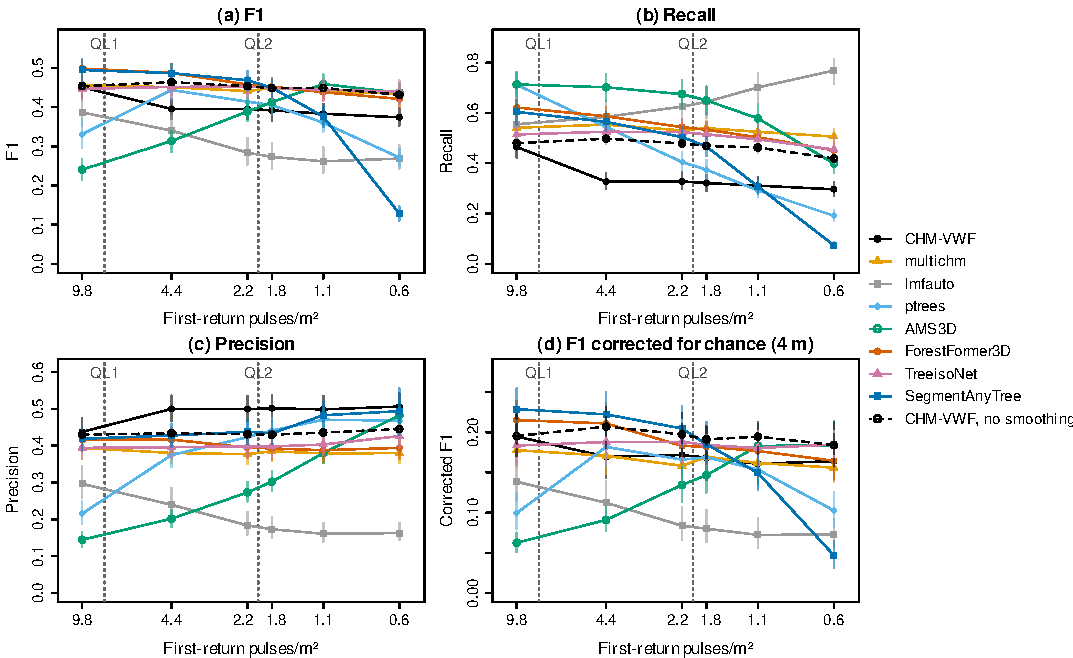
\includegraphics[width=\textwidth]{figures/figure_3.pdf}
\caption{(a) F1, (b) recall, (c) precision and (d) F1 corrected for chance
agreement at the 4 m radius (Section~\ref{sec:4.2}) against the median first-return pulse
density of the plot cores, five sites, nominal plot core, with 95\%
plot-bootstrap intervals; the QL2 level is included. Dotted lines mark the QL1
(8 pulses/m\textsuperscript{2}) and QL2 (2 pulses/m\textsuperscript{2}) floors. The dashed line with open circles is
CHM-VWF run without its smoothing below 8 pulses/m\textsuperscript{2} (Section~\ref{sec:5.2}, Table~S16),
with its interval in (d).}
\label{fig:3}
\end{figure}

The native ranking carries over to the QL2 level and breaks below it (Fig.~\ref{fig:4}).
The Spearman correlation with the native ranking is 0.83, 0.76 and 0.71 [0.38,
0.81] at 4.4, 2.2 and 1.8 pulses/m\textsuperscript{2}, and $-$0.05 [$-$0.17, 0.26] and $-$0.19 at 1.1
and 0.6 pulses/m\textsuperscript{2} (Section~S13). The break appears inside censused subplots
(Table~S13) and survives the chance correction at 4 m (Table~S12g). At 2 m,
however, the corrected correlation at the QL2 level falls to 0.36 [$-$0.02, 0.67],
so the carry-over to that level holds in observed and 4 m corrected F1 only. Two
detectors, singled out after seeing the results, carry the break. One is
SegmentAnyTree; the other is AMS3D, which runs with fixed literature settings
and rises from last at native density to a nominal first at 1.1 pulses/m\textsuperscript{2}.
Without both, the other six correlate with their native ranking at 0.54 at the
two sparsest levels. Six detectors reach that value by chance in 15\% of
orderings, so the statement that they keep their order is weak. The ranking
fails because single detectors move by 0.1 to 0.4 F1.

\begin{figure}[!htbp]
\centering
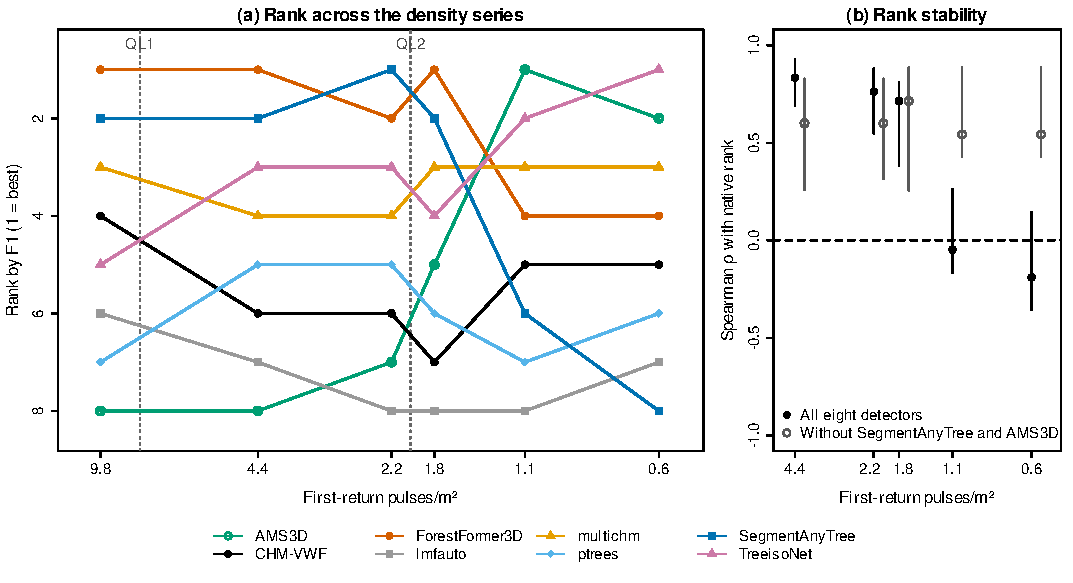
\includegraphics[width=\textwidth]{figures/figure_4.pdf}
\caption{(a) Rank by F1 of the eight detectors run at every density, at
each density level. (b) Spearman correlation between the ranking at native
density and the ranking at each density level, with 95\% plot-bootstrap
intervals, for all eight detectors and for the six left when SegmentAnyTree and
AMS3D are removed; the open circles are drawn slightly to the right of their
level.}
\label{fig:4}
\end{figure}

\subsection{Regions}\label{sec:5.3}

Site sets the level of accuracy more than the choice among the leading detectors
does. Native F1 runs from 0.33 at SJER to 0.54 at ABBY for ForestFormer3D and
from 0.31 to 0.56 for CHM-VWF (Table~S2). SJER, the open woodland, has the
lowest F1 for every detector although recall there is 0.53 to 0.98 among the
LiDAR detectors; its cores hold 59 mapped stems per hectare, and 92 of CHM-VWF's
98 isolated false positives there are co-detected by two other families, so its
F1 is set by reference coverage rather than by detection (Section~S19). Of its
57 reference records, 27 are additional boles of multi-stemmed trees, which one
tree top cannot all match (Section~S14).

On the nominal cores the regions differ in how much of the segmenters' lead lies
above chance (Section~S19, Table~S19). In observed F1 the two segmenters lead
the baseline by about 0.09 in California and, narrowly, by 0.03 in Washington,
where the lead holds at 4 m only: at 3 m and 2 m its intervals include zero
(Section~S21). Every detector scores higher in Washington and the baseline gains
more than the segmenters; for both segmenters the difference between the regions
excludes zero, for SegmentAnyTree narrowly. Corrected for chance on the nominal
cores, their leads are clear in California, +0.060 [+0.026, +0.094] for
ForestFormer3D and +0.061 [+0.015, +0.103] for SegmentAnyTree, and
indistinguishable from zero in Washington, +0.004 [$-$0.026, +0.029] and +0.017
[$-$0.014, +0.042], where Li 2012 is level with them. The Washington estimate is
carried by ABBY ($-$0.043 and $-$0.002), where shifted detections reach at least
four fifths of each detector's F1; at WREF both corrected leads are about +0.03,
with intervals that touch zero (Table~S12f).

Inside censused subplots the contrast does not appear at 4 m. SegmentAnyTree's
corrected lead is +0.067 [$-$0.042, +0.167] on the twelve censused California
plots and +0.058 [+0.005, +0.105] on the 45 Washington plots, where it narrowly
excludes zero under the headline exclusion rule and not under the stricter rule
(+0.046 [$-$0.017, +0.097]) or without the nine plots with a reference outside the
core (+0.040 [$-$0.017, +0.088]). ForestFormer3D's is +0.034 and +0.030, with
intervals that include zero in both regions (Table~S12i). At 2 m both segmenters
lead in California, by +0.076 and +0.064, and neither in Washington (+0.026 and
+0.002); the difference between the regions was not tested inside censused
subplots. With two or three sites per region, held fixed in the bootstrap, these
are contrasts between these sites. The nominal one is not detectable below
native density: at 4.4 pulses/m\textsuperscript{2} the corrected leads are similar in the two
regions (Table~S12d), because CHM-VWF loses 0.07 F1 in Washington at its switch
to the smoothed canopy model. Washington thus reproduces the direction of the
observed leads under settings fixed in advance, narrowly and with smaller leads
than California. Above chance it gives SegmentAnyTree a lead inside censused
subplots at 4 m that narrowly excludes zero under the headline exclusion rule
and not in its sensitivity checks, and neither segmenter a lead on the nominal
cores or at 2 m.

\texttt{multichm} and DeepForest lead the baseline in California and not in Washington,
and Li 2012 is narrowly behind it in California and narrowly ahead in
Washington. DeepForest's California lead does not follow its two training sites:
it leads by as much at SOAP, not a training site, as at TEAK, and trails the
baseline at SJER (Table~S2).

\subsection{Understory trees}\label{sec:5.4}

The point-clustering detectors and ForestFormer3D recall the most understory
stems, and randomly shifted copies of the detections reach most of each
detector's understory recall at 4 m. At native density the nine LiDAR detectors
recall 0.55 to 0.79 of the 1,872 overstory stems and 0.17 to 0.63 of the 592
understory stems (Fig.~\ref{fig:5}; Table~S1; height
bands in Table~S17): AMS3D, \texttt{ptrees} and ForestFormer3D 0.63, 0.46 and 0.45 of
the understory stems, SegmentAnyTree 0.29 and CHM-VWF 0.17. Understory recall
falls with density for most detectors; at 0.6 pulses/m\textsuperscript{2} ForestFormer3D keeps
0.23 and SegmentAnyTree 0.03.

Shifted detections reach 79 to 97\% of each detector's understory recall at 4 m,
against 68 to 80\% of its overstory recall, since an understory stem of 10 m
accepts any detection between 5 and 18 m high within 4 m. Above the null, AMS3D
and ForestFormer3D recall 0.094 of the understory stems and SegmentAnyTree
0.061, while CHM-VWF, TreeisoNet and Li 2012 are indistinguishable from zero at
4 m. At 2 m, where chance matches are rarer, AMS3D recalls 0.15 above the null,
ForestFormer3D 0.11 and most other detectors 0.04 to 0.06, CHM-VWF included.
Every match within 2 m is also a match within 4 m, so the 4 m subtraction also
removes real understory matches of the canopy-surface detectors.
ForestFormer3D's understory advantage over the baseline survives subtraction of
the null, +0.078 [+0.037, +0.119] at 4 m against +0.284 observed.

\begin{figure}[!htbp]
\centering
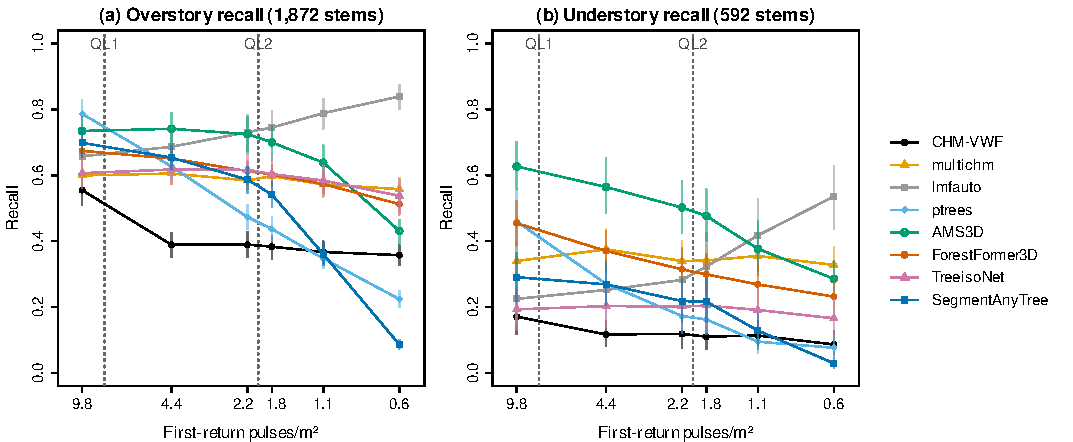
\includegraphics[width=\textwidth]{figures/figure_5.pdf}
\caption{Recall of (a) overstory (dominant and codominant) and (b)
understory (intermediate and suppressed) stems against median first-return pulse
density, five sites, with 95\% intervals.}
\label{fig:5}
\end{figure}

\subsection{Reference completeness}\label{sec:5.5}

Scoring inside censused subplots raises every detector's precision and widens,
rather than narrows, the segmenters' leads. On the 57 admitted plots it raises
precision by 0.08 to 0.34 for every detector and density, while recall moves by
at most 0.03; CHM-VWF's native precision rises from 0.48 to 0.78 (Table~\ref{tab:5};
Section~S20, Fig.~S1). Detectors with dense apexes keep a low censused
precision, 0.24 for AMS3D, so most of their commission is not explained by
unsampled area.

Inside censused subplots SegmentAnyTree and ForestFormer3D lead CHM-VWF by
+0.068 and +0.059 at native density, against +0.041 and +0.026 in the nominal
cores of the same plots (Table~\ref{tab:5}). CHM-VWF gains the most precision, but its F1
stays held by its recall. ForestFormer3D's lead over Li 2012 is no longer
distinguishable from zero, while SegmentAnyTree's remains, narrowly, and Li
2012's own censused lead over the baseline excludes zero. The censused table
rests mostly on the Washington sites, which hold 1,055 of its 1,190 references.

Chance agreement is as large inside censused subplots as on the nominal cores,
and the corrected leads are larger. Shifted copies of the detections, scored by
the censused scorer, reach 72 to 83\% of each detector's censused F1 (Table~\ref{tab:5}).
SegmentAnyTree's corrected lead over CHM-VWF is +0.063 [+0.016, +0.108], twice
its corrected lead in the nominal cores of the same plots. It holds at 2 m,
narrowly (+0.034 [+0.006, +0.063]). Two sensitivities bring its lower limit to
zero: under the stricter exclusion rule the interval just includes it (+0.052
[$-$0.002, +0.100]), and without nine plots whose references reach outside the
nominal core it narrowly excludes it (+0.052 [+0.002, +0.098]; Section~S12).
ForestFormer3D's, +0.030 [$-$0.016, +0.074], and Li 2012's, +0.025 [$-$0.004,
+0.057], include zero, and \texttt{multichm} falls behind the baseline. In corrected
recall the two segmenters lead the baseline by 0.113 and 0.102, as on the
nominal cores, and in corrected precision they trail it by 0.095 and 0.161. In
the corrected scores, then, the segmenters lead in recall and trail in
precision, and the balance favours SegmentAnyTree clearly and ForestFormer3D not
distinguishably. A lead that doubles from the nominal cores to the censused
subplots is what the simulation gives for a real difference in skill when half
of a core holds no reference, for observed and corrected leads alike (Section~S27), and part of it is scale, since every detector's corrected F1 is higher
inside censused subplots. The plot types, split post hoc, do not show that
mechanism, however. On the 54 distributed plots, whose core is a single 20 m
subplot, the nominal-core corrected leads of SegmentAnyTree and ForestFormer3D
are +0.022 and +0.027, with intervals that include zero on a third of the stems,
and on the half-mapped tower plots SegmentAnyTree's is larger, +0.042, and
ForestFormer3D's only slightly smaller, +0.021 (Table~S12k).

The co-detection credit raises F1 by 0.07 to 0.14 per detector at its best
density per site and leaves the two segmenters in the lead (Table~S5). Both
brackets point the same way: nominal-plot precision understates every detector,
and inside censused subplots the baseline most (Section~S20).

\begin{sidewaystable}
\centering
{\footnotesize
\setlength{\tabcolsep}{3pt}
\renewcommand{\arraystretch}{1.15}
\begin{tabularx}{\linewidth}{>{\hsize=1.18\hsize\linewidth=\hsize}L>{\hsize=1.01\hsize\linewidth=\hsize}L>{\hsize=1.08\hsize\linewidth=\hsize}L>{\hsize=0.68\hsize\linewidth=\hsize}L>{\hsize=0.96\hsize\linewidth=\hsize}L>{\hsize=1.08\hsize\linewidth=\hsize}L>{\hsize=0.68\hsize\linewidth=\hsize}L>{\hsize=1.01\hsize\linewidth=\hsize}L>{\hsize=1.13\hsize\linewidth=\hsize}L>{\hsize=1.19\hsize\linewidth=\hsize}L}
\toprule
Detector & Nominal F1, same plots & Nominal lead & Censused precision & Censused F1 & Censused lead & Censused null F1 & Censused corrected F1 & Censused corrected lead & Nominal corrected lead, same plots \\
\midrule
SegmentAnyTree & 0.528 [0.503, 0.555] & +0.041 [+0.018, +0.066] & 0.718 & 0.677 [0.644, 0.708] & +0.068 [+0.036, +0.100] & 0.490 & 0.366 [0.324, 0.409] & +0.063 [+0.016, +0.108] & +0.029 [+0.000, +0.059] \\
ForestFormer3D & 0.513 [0.490, 0.539] & +0.026 [$-$0.000, +0.053] & 0.675 & 0.668 [0.640, 0.695] & +0.059 [+0.020, +0.099] & 0.502 & 0.333 [0.285, 0.385] & +0.030 [$-$0.016, +0.074] & +0.000 [$-$0.030, +0.030] \\
Li 2012 & 0.506 [0.481, 0.531] & +0.018 [+0.005, +0.032] & 0.692 & 0.638 [0.599, 0.676] & +0.030 [+0.011, +0.049] & 0.462 & 0.328 [0.287, 0.371] & +0.025 [$-$0.004, +0.057] & +0.016 [+0.000, +0.034] \\
TreeisoNet & 0.488 [0.465, 0.512] & +0.001 [$-$0.015, +0.015] & 0.720 & 0.622 [0.581, 0.663] & +0.013 [$-$0.009, +0.034] & 0.457 & 0.303 [0.261, 0.346] & +0.000 [$-$0.033, +0.030] & $-$0.005 [$-$0.028, +0.014] \\
CHM-VWF & 0.487 [0.463, 0.514] & --- & 0.779 & 0.608 [0.566, 0.651] & --- & 0.438 & 0.303 [0.260, 0.346] & --- & --- \\
\texttt{multichm} & 0.468 [0.448, 0.493] & $-$0.020 [$-$0.043, +0.006] & 0.636 & 0.597 [0.570, 0.626] & $-$0.011 [$-$0.047, +0.026] & 0.456 & 0.260 [0.220, 0.305] & $-$0.043 [$-$0.082, $-$0.008] & $-$0.038 [$-$0.061, $-$0.014] \\
\texttt{lmfauto} & 0.403 [0.365, 0.452] & $-$0.084 [$-$0.121, $-$0.039] & 0.492 & 0.539 [0.494, 0.594] & $-$0.070 [$-$0.117, $-$0.017] & 0.401 & 0.229 [0.180, 0.294] & $-$0.073 [$-$0.127, $-$0.012] & $-$0.067 [$-$0.097, $-$0.030] \\
\texttt{ptrees} & 0.355 [0.314, 0.403] & $-$0.132 [$-$0.177, $-$0.082] & 0.372 & 0.496 [0.439, 0.554] & $-$0.113 [$-$0.181, $-$0.046] & 0.389 & 0.175 [0.114, 0.245] & $-$0.128 [$-$0.201, $-$0.058] & $-$0.104 [$-$0.142, $-$0.067] \\
AMS3D & 0.263 [0.238, 0.291] & $-$0.225 [$-$0.254, $-$0.191] & 0.243 & 0.364 [0.322, 0.404] & $-$0.245 [$-$0.298, $-$0.188] & 0.300 & 0.090 [0.060, 0.126] & $-$0.212 [$-$0.257, $-$0.166] & $-$0.148 [$-$0.179, $-$0.119] \\
\bottomrule
\end{tabularx}
}
\caption{Censused subplots at native density (57 plots, 1,190 censused
references) beside the nominal plot core on the same 57 plots (1,607 stems),
with 95\% intervals; leads are over CHM-VWF, with paired intervals. Null F1,
corrected F1 and corrected lead: the shift null scored inside the censused
subplots at 4 m; the last column is the corrected lead in the nominal cores of
the same plots. The RGB detectors are not in the censused scorer.}
\label{tab:5}
\end{sidewaystable}

\subsection{Decimation against native sparse flights}\label{sec:5.6}

Thinning is optimistic against natively sparse flights, mildly for most
detectors and strongly for SegmentAnyTree's recall. The 2017 and 2018 flights
give lower recall than both thinned 2021 levels, the one close to them in
density and the one half as dense, for every detector (Fig.~\ref{fig:6}). For CHM-VWF,
\texttt{multichm}, ForestFormer3D and TreeisoNet the gap is 0.03 to 0.05, with most
intervals excluding zero, and ForestFormer3D's F1 on the sparse flights is level
with both levels. SegmentAnyTree's recall on the sparse flights, 0.42, is 0.193
[0.156, 0.231] below the level at about 4.9 pulses/m\textsuperscript{2} and 0.063 [0.012, 0.119]
below the level at about 2.5 pulses/m\textsuperscript{2}. In F1 its gap is like the others', and
on the sparse flights its F1 (0.40) equals \texttt{multichm}'s and exceeds the
baseline's (0.33). Its recall on thinned clouds is therefore likely optimistic,
and the density at which it falls behind on a native acquisition may be higher
than Table~\ref{tab:4} suggests. The comparison cannot separate thinning from the other
differences between the epochs (Section~\ref{sec:4.6}). The cross-sensor check agrees for
both detectors run on it: between 3DEP and NEON clouds both thinned to 2
points/m\textsuperscript{2} (about 1.2 pulses/m\textsuperscript{2} in the plot cores), CHM-VWF differs by $-$0.026
[$-$0.057, +0.006] F1 and \texttt{multichm} by $-$0.015 [$-$0.037, +0.009].

\begin{figure}[!htbp]
\centering
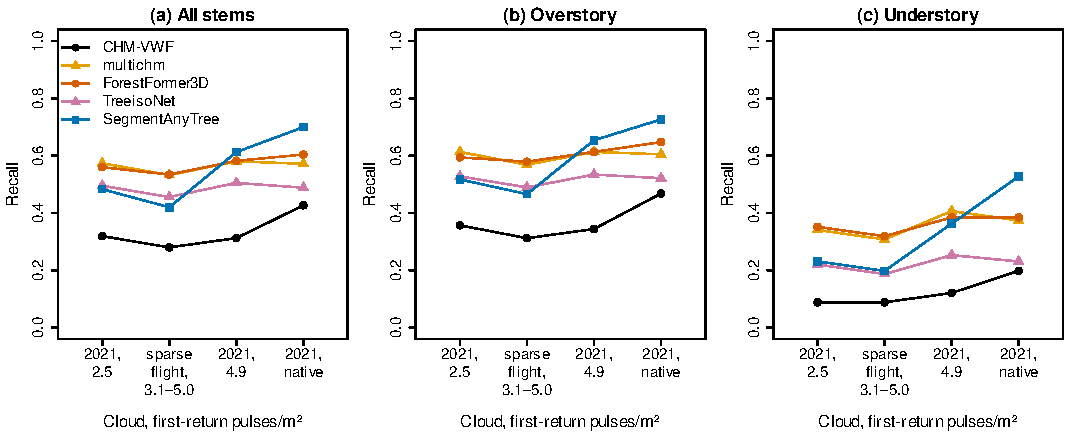
\includegraphics[width=\textwidth]{figures/figure_6.pdf}
\caption{Recall on the natively sparse 2017 and 2018 flights and on the
2021 clouds at two thinned density levels and at native density, for the 586
stems live in both epochs on 39 California plots: (a) all stems, (b) overstory
and (c) understory. Densities are medians inside the cores of these plots: 4.6
pulses/m\textsuperscript{2} for the sparse flights (3.1 to 5.0 by site), and 4.9 and 2.5 for the
two thinned levels, which are denser on these plots than over the five sites.
Differences with paired intervals are given in the text.}
\label{fig:6}
\end{figure}

\subsection{Dense-domain control}\label{sec:5.7}

On dense data with complete labels the same checkpoints and adapters work, and
they lead the baseline far more than on NEON. On the FGI-EMIT reserve
ForestFormer3D and SegmentAnyTree reach apex F1 of 0.78 and 0.75, against 0.49
for CHM-VWF (Table~\ref{tab:6}), and mask F1 of 0.65 and 0.58 against the manual labels.
These mask scores are close to, though below, the 0.73 and 0.65 that the dataset
authors report for the same architectures trained on FGI-EMIT and scored on
other plots \citep{ruoppa2026benchmarking}, which is context and not a like-for-like
comparison. The leads of 0.26 to 0.29 are point estimates on three plots.

Density accounts for the contrast with NEON only for ForestFormer3D, and only at
NEON's native density. Thinned to 11.3 pulses/m\textsuperscript{2}, the level paired with native
NEON, ForestFormer3D's lead on the development plots falls from 0.30 to 0.08,
with an interval that overlaps that of its NEON lead of 0.05. From 5.4 pulses/m\textsuperscript{2}
down, however, it leads by 0.17 to 0.21 on FGI-EMIT against 0.05 to 0.09 on
NEON, partly because the baseline loses 0.14 on FGI-EMIT at its switch to the
smoothed canopy model and 0.06 on NEON. SegmentAnyTree's lead stays above the
NEON level at every density above its collapse. That collapse replicates against
true labels: on thinned FGI-EMIT SegmentAnyTree's lead holds to 2.9 pulses/m\textsuperscript{2},
vanishes at 1.5 and reverses at 0.7. Under the 40-point instance filter of the
policy fixed on the development plots, the two segmenters keep 4 and 1
detections at 0.7 pulses/m\textsuperscript{2} over the ten plots, against 378 and 56 under the
apex rule. Their scores on sparse clouds thus depend on post-processing fitted
to dense clouds.

The control also exposed one of two integration defects that had looked like
domain shift and raised no error. ForestFormer3D's first NEON runs scored F1
0.23 to 0.33 on the California sites, because file names selected an upstream
fallback route and tiled instances were merged by apex proximity. With the route
corrected and whole-scene inference, its F1 on the two FGI-EMIT audit plots rose
from 0.09 to 0.75, and on the same NEON plots to 0.33 to 0.50. TreeisoNet, which
has no such control, had scored 0.08 and 0.12 at two California sites because
its voxel setting differed between sites, a defect caught only by comparing
sites; with the airborne setting it scores 0.28 and 0.37 there, in sample
(Section~\ref{sec:4.5}).

\begin{sidewaystable}
\centering
{\footnotesize
\setlength{\tabcolsep}{3pt}
\renewcommand{\arraystretch}{1.15}
\begin{tabularx}{\linewidth}{lllLLLLLL}
\toprule
Plots & Pulses/m\textsuperscript{2} & CHM-VWF & ForestFormer3D & SegmentAnyTree & ForestFormer3D lead & ForestFormer3D lead on NEON & SegmentAnyTree lead & SegmentAnyTree lead on NEON \\
\midrule
Reserve & native & 0.488 & 0.776 & 0.746 & +0.288 & --- & +0.258 & --- \\
Development & native & 0.513 & 0.811 & 0.729 & +0.298 [+0.181, +0.385] & --- & +0.216 [+0.110, +0.288] & --- \\
Development & 11.3 & 0.507 & 0.590 & 0.666 & +0.083 [+0.034, +0.126] & +0.048 [+0.028, +0.069] & +0.159 [+0.092, +0.206] & +0.044 [+0.021, +0.067] \\
Development & 5.4 & 0.366 & 0.569 & 0.605 & +0.203 [+0.174, +0.229] & +0.092 [+0.065, +0.120] & +0.239 [+0.196, +0.276] & +0.091 [+0.064, +0.117] \\
Development & 2.9 & 0.354 & 0.565 & 0.543 & +0.210 [+0.175, +0.243] & +0.062 [+0.035, +0.088] & +0.189 [+0.156, +0.221] & +0.073 [+0.046, +0.099] \\
Development & 1.5 & 0.361 & 0.544 & 0.393 & +0.184 [+0.143, +0.218] & +0.055 [+0.029, +0.079] & +0.032 [$-$0.036, +0.096] & $-$0.007 [$-$0.030, +0.016] \\
Development & 0.7 & 0.344 & 0.515 & 0.116 & +0.171 [+0.127, +0.214] & +0.047 [+0.022, +0.069] & $-$0.228 [$-$0.308, $-$0.162] & $-$0.246 [$-$0.268, $-$0.223] \\
\bottomrule
\end{tabularx}
}
\caption{Apex F1 on FGI-EMIT. Reserve: three plots, 257 trees, native
density, under the 40-point instance filter of the policy fixed on the
development plots. Development: ten plots, 841 trees, thinned to the NEON
densities, under the 2 m apex rule (the two rules differ by at most 0.003 at
native density). Leads are over CHM-VWF, with 95\% intervals on the development
plots; the NEON columns give the five-site observed lead at the corresponding
density level, scored without the 2 m apex floor.}
\label{tab:6}
\end{sidewaystable}

\section{Discussion}\label{sec:6}

\subsection{Choosing a detector by USGS quality level}\label{sec:6.1}

The density series and a decision table built from it answer RQ4 as guidance
for a user of national-mapping LiDAR. The table (Section~S25) places every cell,
one plot at one density level, in a band by the first-return density of its plot
core, and in each band picks the detector with the highest pooled F1 on the
California cells, among the eight detectors run at every density with a GPU or
the five classical ones with only a CPU; the Washington cells check each pick
(Table~S25a). With a GPU it picks SegmentAnyTree from the QL2 floor up and
\texttt{multichm} below it, and with only a CPU \texttt{multichm} in every band. Three
cautions apply. The table was designed after the results were known. Its GPU
picks above the floor lead ForestFormer3D by 0.009 and 0.002 F1 on the
development data, with intervals that include zero and margins of the size of
the run-to-run variation measured for ForestMamba (0.007 F1; Section~S23). And
the pick between the floors changes with the definition of density.

At QL1 density or denser, at least 8 pulses/m\textsuperscript{2}, a user with a GPU can run either
segmenter: SegmentAnyTree is the pick and the Washington best, and
ForestFormer3D is level with it. Their observed lead over the canopy-model
baseline, 0.04 to 0.05 F1 at 4 m, costs 30 to 140 times the baseline's compute
(Table~\ref{tab:2}). In the corrected scores they lead the baseline by about a tenth in
recall and do not lead it in precision; in corrected F1 the balance is 0.02 to
0.03 on the nominal cores and 0.03 to 0.06 inside censused subplots, where only
SegmentAnyTree's lead excludes zero. With only a CPU, either canopy-model
detector serves: \texttt{multichm} was the California pick, but the baseline scored
higher in Washington, narrowly in F1, by 0.035, and by 0.056 in corrected F1.

Between the QL2 and QL1 floors, 2 to 8 pulses/m\textsuperscript{2}, the two segmenters are level
on thinned clouds, and the table's pick turns on 0.002 F1. We would run
ForestFormer3D there. SegmentAnyTree lost almost a quarter of its recall by the
QL2 level, and on native sparse flights at 3 to 5 pulses/m\textsuperscript{2} its recall was 0.19
below a level thinned to about the same density and 0.06 below one half as
dense, so we would not rely on it near QL2 without a check at that density. With
only a CPU the choice is between \texttt{multichm} and the baseline run without its
smoothing, a post hoc configuration that was not a candidate of the table and
has no held-out check; the two score within 0.013 F1 of each other on every
thinned level (Table~S16). The regions disagree on them: \texttt{multichm} leads the
unsmoothed baseline by 0.04 to 0.05 F1 in California, and in Washington it
trails it in corrected F1, by 0.04 to 0.07 on every thinned level, and by 0.02
to 0.04 in observed F1, where the interval excludes zero on two levels. The
0.057 to 0.060 F1 by which the four leading detectors beat the smoothed baseline
at the QL2 level reflects that rule more than their skill: against the
unsmoothed baseline their leads there are +0.001 to +0.004, and above chance
none leads it on any thinned level of the five sites, on the nominal cores or
inside censused subplots. The rule costs the baseline accuracy in Washington
only: in California ForestFormer3D still leads the unsmoothed baseline above
chance at 4.4 pulses/m\textsuperscript{2}, and SegmentAnyTree narrowly at 4.4 and 2.2 (Section~S16).

Below the QL2 floor, under 2 pulses/m\textsuperscript{2}, SegmentAnyTree should not be run, and in
observed F1 a CPU detector is enough. With a GPU the table itself picks
\texttt{multichm}, which in Washington is level with ForestFormer3D, TreeisoNet and
AMS3D; in corrected F1, TreeisoNet registers to the mapped stems better, by
0.043, and ForestFormer3D and AMS3D narrowly better. Below the floor a
detector's score at native density does not guarantee its score. SegmentAnyTree,
one of the two best at 10 pulses/m\textsuperscript{2}, is the worst at 0.6, and AMS3D, the worst
at 10 pulses/m\textsuperscript{2}, is level with the best three at 1.1. These cells are thinned
copies of denser clouds, which the native-flight check found optimistic, and no
native acquisition at or below QL2 density covers the plots. A detector for such
data has to be chosen from an evaluation at that density.

A single detector is a simpler choice. With a GPU, ForestFormer3D run at every
density is level with the table's picks, which lead it by +0.003 [$-$0.006,
+0.012] F1 over every cell of the five sites and trail it by 0.003 in Washington
(Table~S25i). What the table adds is a rule that keeps SegmentAnyTree off clouds
below the floor, where \texttt{multichm} beats it by 0.080 [0.058, 0.103] F1 in
Washington (Table~S25g). With only a CPU, the table picks \texttt{multichm}
throughout. Licences also bear on the choice: ForestFormer3D's
code and TreeAIBox are released for non-commercial use (CC BY-NC 4.0), while
SegmentAnyTree is under the MIT licence and the classical detectors under
GPL-3.0 (Section~S11). Fusing detectors buys little: at native density no
fused mode beats the best single detector, and at sparser densities agreement of
two detectors gains 0.01 to 0.02 F1 with a threshold chosen in sample (Section~S6). For understory trees, the detectors that recall the most stems split the
point cloud aggressively, at a precision of 0.15 to 0.22, while ForestFormer3D's
recall above the null comes at a precision of 0.42. Since two thirds of the
understory reference is at one old-growth site, understory recall should be
re-measured where understory stems are censused more widely, with a tighter
radius and a chance null.

\subsection{Why one learned detector collapses}\label{sec:6.2}

Fig.~\ref{fig:7} shows the collapse on one typical plot. From native density to the
sparsest level CHM-VWF and ForestFormer3D keep most of their matches, while
SegmentAnyTree's detections in the core fall from 55 to 5.

\begin{figure}[!htbp]
\centering
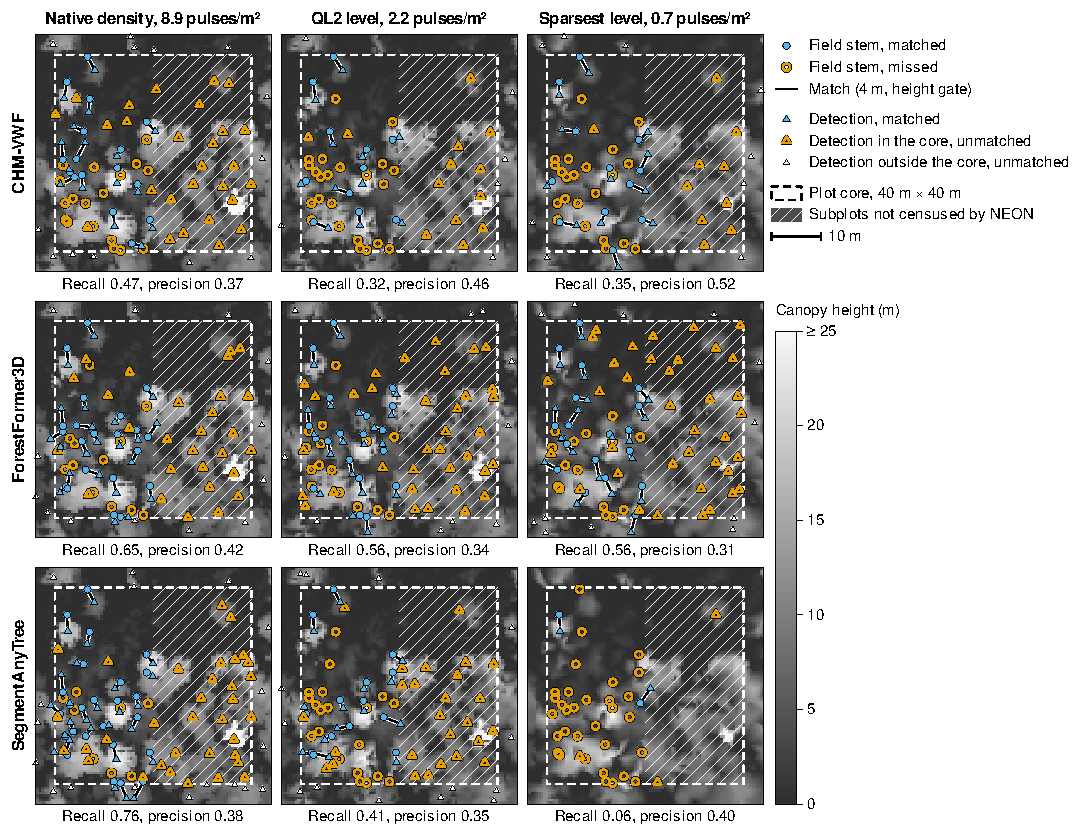
\includegraphics[width=\textwidth]{figures/figure_7.pdf}
\caption{Detections by CHM-VWF, ForestFormer3D and SegmentAnyTree on one
tower plot at SOAP, at native density, at the QL2 level and at the sparsest
density level; the column headings give the first-return density of the plot's
core at each level, against five-site medians of 9.8, 1.8 and 0.6 pulses/m\textsuperscript{2}.
Circles are the field stems of the 40 m $\times$ 40 m plot core (dashed) and triangles
the detections: filled blue when matched, open orange when a stem is missed or a
detection in the core is unmatched; small white triangles are unmatched
detections in the 4 m margin, which are not scored. NEON censused two of the
plot's four 20 m subplots, the western half, which holds all 34 reference stems;
in the hatched eastern half no stem is mapped, and every core detection there
counts against precision in the nominal-core score (Section~\ref{sec:4.3}). Lines join
matched pairs (Section~\ref{sec:4.2}). Background: canopy height model of each level's
fixed evaluation clip, on one grey scale for all panels. Recall and precision of
this plot are given under each panel. The plot was chosen by a fixed rule: among
the plots with at least 10 reference stems and at least one core detection in
every one of the nine panels, it is the plot whose nine F1 values lie closest,
by Euclidean distance, to the five-site pooled F1 of the same detectors and
levels, so it is typical rather than extreme.}
\label{fig:7}
\end{figure}

The collapse belongs to SegmentAnyTree at these densities, on two datasets and
against two kinds of reference, and not to learned detectors as a family; it
survives the chance correction and the change of baseline. SegmentAnyTree's
released checkpoint was trained with sparsified copies, down to 10 points/m\textsuperscript{2} of
all returns \citep{wielgosz2024segmentanytree,ruoppa2026benchmarking}. Its collapse
sets in below about a third of that density (3.2 points/m\textsuperscript{2} at the QL2 level,
Section~S15) and is complete at a tenth, so it is a failure below the training
range rather than within it. Its authors report a drop at 10 points/m\textsuperscript{2}, their
sparsest training density, driven by omission \citep{wielgosz2024segmentanytree}, and
the FGI-EMIT authors found its F1 stable to that density
\citep{ruoppa2026benchmarking}. The other two were trained on dense data, as far as
their sources say. ForestFormer3D's paper states no training density; it reports
that a variant retrained with SegmentAnyTree's multi-density copies improved
below 100 points/m\textsuperscript{2}, without saying which variant was released
\citep{xiang2025forestformer3d}. TreeAIBox's wellsite models are described on
unmanned scans of about 1,160 points/m\textsuperscript{2} \citep{movchan2025uavbased}. Both degrade
gracefully. The persisted outputs locate the failure (Table~S18a). From native
density to 0.6 pulses/m\textsuperscript{2} SegmentAnyTree's semantic head still labels 70 to 89\%
of the core points as tree, but the share of those points grouped into an
instance falls from 0.86 to 0.05 and the mean core instance from 272 to 13
points, while ForestFormer3D keeps 0.67 to 0.55 of its core points in instances:
its mask decoder, which keeps instances of at least 10 points, degrades with the
point count instead. In SegmentAnyTree the grouping stage fails, not the learned
semantics, and not through its fixed 0.3 m search radius alone: in a post hoc
check on ten California plots at 1.1 and 0.6 pulses/m\textsuperscript{2}, radii of 1.5 and 3 times
the point spacing changed F1 by $-$0.02 to +0.03, within intervals that include
zero, and the larger merged neighbouring trees (Section~S18). The coarse voxels
of TreeisoNet's localisation pass aggregate sparse returns, consistent with its
flat response. Ablations by the model authors would settle the mechanisms.

\subsection{The dense benchmark and integration defects}\label{sec:6.3}

The segmenters lead the baseline by 0.26 to 0.29 F1 on FGI-EMIT and by about
0.05 on NEON, and density accounts for the difference only for ForestFormer3D at
NEON's native density (Section~\ref{sec:5.7}). The baseline's response to its rule switch,
the completeness of the labels, the forests, the acquisitions and the apex
matchers all differ between the two datasets, and the design cannot separate
them; the chance null, which reproduces most of the nominal-core NEON leads, was
not computed on FGI-EMIT. We therefore report a contrast between two datasets,
not a law for the size of the lead.

Two of the three learned detectors were at first misjudged by a wide margin
because of an adapter and a configuration value, and neither produced an error.
A zero-shot benchmark that reports a published model failing on new data should
therefore show the same code path succeeding where the model is known to work,
as ecological assessments of transferability report accuracy within the fitting
data beside accuracy on new data \citep{wenger2012assessing,yates2018outstanding};
we could do so for two of the three detectors. The practical rules are to run
ForestFormer3D on whole scenes within GPU memory, never to merge tiled instances
by apex proximity, and to check that post-processing fitted to dense clouds,
such as a minimum of 40 points per instance, does not remove the detections on
sparse ones.

\subsection{Threats to validity}\label{sec:6.4}

\begin{table}[!htbp]
\centering
{\footnotesize
\setlength{\tabcolsep}{3pt}
\renewcommand{\arraystretch}{1.15}
\begin{tabularx}{\linewidth}{>{\hsize=0.93\hsize\linewidth=\hsize}L>{\hsize=1.56999\hsize\linewidth=\hsize}L>{\hsize=0.50\hsize\linewidth=\hsize}L}
\toprule
Issue & Direction of bias & Where tested \\
\midrule
Incomplete reference: unmapped or uncensused trees, half of each tower core unsampled; stems measured up to four years from the flight, on three SOAP plots only before a fire & Lowers every detector's precision, the baseline's most; in simulation an unsampled half of a core lowers a real F1 lead, and inside censused subplots the segmenters' leads widen; ForestFormer3D's lead vanishes on flight-year stems; leaving out the fire plots changes little & Sections~\ref{sec:4.3}, \ref{sec:5.1}, \ref{sec:5.5}, S4, S5, S12, S14, S20, S21 and S27 \\
A 4 m match radius admits chance matches; the shift null is not an estimate of the chance part of a score & Raises every F1, shifted copies reaching 70 to 79\% of native F1; in simulation corrected F1 leads understate a difference in skill when the extra detections are of the leader's own trees or uniform and overstate it when they lie beside trees (unmapped trees, split crowns), and corrected recall credits extra detections; the segmenters split crowns at about half the simulated rate or less, enough for part of their recall lead, and where the unmapped trees stand is not measured & Sections~\ref{sec:4.2}, \ref{sec:5.1}, S12, S21, S27 and S28 \\
Thinning instead of native sparse acquisitions; one seed per density level & Optimistic, mildly for four detectors and strongly for SegmentAnyTree's recall, untested at or below QL2; seed spread measured for the baseline only & Sections~\ref{sec:3.3}, \ref{sec:3.4} and \ref{sec:5.6} \\
The baseline's pre-declared smoothing rule & Costs it about 0.06 F1 and 0.02 to 0.04 corrected F1 on the thinned levels, inflating the leads over it & Sections~\ref{sec:5.2} and S16 \\
Settings developed in California; chance null, censused null, unsmoothed baseline, core densities, the simulation of the correction, the split-crown count and the decision table of Section~\ref{sec:6.1} added post hoc & Favour California scores, Washington held out; choices not blind to Washington, the table's picks selected on California only, and its pick between the QL2 and QL1 floors changes with the definition of density & Sections~\ref{sec:4.5}, \ref{sec:4.7}, \ref{sec:5.3}, \ref{sec:6.1}, S11, S19, S25, S26, S27 and S28 \\
Pooling weights sites by stems, Washington holding 74\%; intervals not adjusted for multiple contrasts & Five-site estimates are mostly Washington estimates; about five of 90 corrected-lead contrasts would exclude zero by chance alone & Sections~\ref{sec:4.4} and S19 \\
Learned detectors inferred once; TreeisoNet's threshold untuned for its voxel, no dense-domain control; Li 2012 run at native density only & Run-to-run variation of ForestFormer3D and TreeisoNet unknown, and of the size of the margins that decide the decision table's picks if it resembles ForestMamba's; TreeisoNet's precision-recall balance, hence its flat response, is that of an arbitrary operating point; Li 2012's density response unknown & Not tested (Sections~\ref{sec:4.1}, \ref{sec:4.4} and \ref{sec:6.1}) \\
DeepForest trained on annotations from SJER and TEAK; checkpoints' training histories incomplete & Could favour DeepForest there, though its California lead does not follow them; overlap with the test data not excluded & Sections~\ref{sec:3.5} and \ref{sec:5.3} \\
Oak woodland and conifer forest in two western regions only; SJER's 31 March flight may precede its blue oaks' full leaf-out & Results may not transfer to closed-canopy broadleaf or deciduous forest & Not tested \\
Mask quality not assessed on NEON & Rankings of masks rest on a proxy reference & Sections~S7 and S8 \\
\bottomrule
\end{tabularx}
}
\caption{Threats to validity: each issue, the direction in which it would
bias the results, and where it is tested.}
\label{tab:7}
\end{table}

Of the threats in Table~\ref{tab:7}, three bear on every conclusion: the reference is
incomplete, so nominal-plot precision is a lower bound and the corrected scores,
which measure agreement beyond shifted copies of the same detections, are not
bounds on skill; every density below native is simulated by thinning, which the
one native comparison, at 3 to 5 pulses/m\textsuperscript{2}, suggests is optimistic; and the
chance null, its censused form, the unsmoothed baseline, the simulation of the
correction, the split-crown count and the decision table were added after the
five-site results were known. The learned detectors are
evaluated zero-shot, as a practitioner would use published checkpoints; NEON
provides stems and not instance labels, so the benchmark says nothing about what
training at these densities could achieve. A fourth learned detector,
ForestMamba \citep{nguyen2026forestmamba}, run after the tables were fixed, fits the
pattern of the result tables: it does not lead the baseline at native density,
does not collapse, and its leads below native density rest on the baseline's
smoothing rule (Section~S23).

\section{Conclusion}\label{sec:7}

At five NEON sites in California and Washington, flown at about 10 pulses/m\textsuperscript{2},
two of three published learned 3D detectors used zero-shot score 0.04 to 0.05 F1
above a canopy-model baseline whose resolution and smoothing follow measured
density, at a 4 m match radius; the third does not lead (RQ1). Randomly shifted
copies of the same detections reach 70 to 79\% of every detector's F1. In
corrected recall the two segmenters lead the baseline by about a tenth, part of
which split crowns produce, and in corrected precision they do not lead it. In
corrected F1 SegmentAnyTree leads by 0.03 on the nominal plot cores and by 0.06
inside censused subplots; in the Washington replication region that lead
narrowly excludes zero at 4 m under the headline exclusion rule and not in its
sensitivity checks. ForestFormer3D's lead of 0.02 to 0.03 does not exclude zero.
A corrected score measures agreement beyond shifted copies of the same
detections. In simulation a corrected F1 lead understates a difference in skill
when the extra detections are of the leader's own trees or uniform and
overstates it when they lie beside trees, and in loose clusters, the simulated
stand nearest to the reference stems of all distributed plots, split crowns at
the segmenters' surplus of detections reproduce their corrected recall lead but
not a positive corrected F1 lead. In the benchmark's own detections the
segmenters split crowns at about half that rate or less, enough for part of the
recall lead, and for a smaller part if the stands are as little clustered as the
reference stems of the distributed plots admitted to censused scoring. The
corrected leads are therefore not bounds on a difference in skill.

Density response is a property of the individual model, not of its family (RQ2):
SegmentAnyTree collapses just below the QL2 floor, between 1.8 and 1.1
pulses/m\textsuperscript{2}, at its instance-grouping stage, while ForestFormer3D and TreeisoNet
degrade gracefully. Below native density the five-site leads of ForestFormer3D,
TreeisoNet and \texttt{multichm} over the baseline rest on its smoothing rule: without
it the baseline is within 0.03 F1 of them, and above chance none of them leads
it, on the nominal cores or inside censused subplots. The rule costs the
baseline accuracy in Washington only, and in California the two segmenters still
lead the unsmoothed baseline above chance at 4.4 pulses/m\textsuperscript{2}. Native-density rank
predicts rank down to the QL2 level and not below it, where two of the eight
detectors move by 0.1 to 0.4 F1 (RQ3).

For users of national-mapping LiDAR (RQ4) we offer guidance, not a tested
pipeline. With a GPU, ForestFormer3D can be run at every density: on the five
sites and in Washington it does as well as a post hoc decision table, selected
on California, that runs SegmentAnyTree from the QL2 floor up and a multi-layer
canopy-model detector below it. SegmentAnyTree should not be run below the
floor, and near it the native sparse flights argue against relying on it without
a check at that density. Without a GPU, a canopy-model detector serves at every
density; below the floor it is level with the best learned detectors in
Washington in observed F1 at 4 m, though not in corrected F1. The sparsest
densities rest on thinned clouds, so a detector for sparse data is still best
chosen from an evaluation at that density.

Five practices made these statements possible and are, we suggest, necessary for
such benchmarks: reporting the score of randomly shifted copies of the
detections, scoring inside censused subplots as well as on nominal plots,
measuring density on the scored area, checking thinning against a native sparse
acquisition, and running a positive control where the models are known to work.
The clips, detections and code are public, and the tables rebuild from them with
one command, so new detectors can join the same tables.


\section*{CRediT authorship contribution statement}
% TODO: complete this section.
To be completed with the author list.

\section*{Declaration of competing interest}
% TODO: complete this section.
To be completed by the authors.

\section*{Funding}
% TODO: complete this section.
To be completed by the authors.

\section*{Data and code availability}
All field, airborne LiDAR and camera data of the benchmark are public data
products of the National Ecological Observatory Network, released under CC0 1.0:
vegetation structure \citep{neon2026vegetation}, the discrete-return LiDAR point
cloud \citep{neon2026discrete} and the camera imagery mosaic \citep{neon2026camera}, from
the 2021 flights over SJER, SOAP, TEAK, WREF and ABBY. The cross-sensor check
also uses public-domain USGS 3DEP point clouds \citep{usgs2026usgs}. The fixed
evaluation clips, field-stem references, plot populations, per-cell results and
persisted detections, checkpoint hashes and container image identifiers are
archived at Zenodo (DOI to be assigned at deposit), with a script that rebuilds
every table from the archive, the density-routing analysis included; the radius
check of Section~S18 and the ForestMamba run of Section~S23 are not in the
archive. The code is available at
\url{https://github.com/devakellc/lidar-tree-benchmark} under the MIT licence.
Third-party models are used under their own licences and are not redistributed;
the archive lists their sources, versions and SHA-256 hashes, and the repository
lists ForestMamba's (Section~S23). FGI-EMIT is available from its authors under
CC BY-NC-SA 4.0 \citep{ruoppa2026fgiemit}.

\section*{Acknowledgements}
The National Ecological Observatory Network is a program sponsored by the U.S.
National Science Foundation and operated under cooperative agreement by
Battelle. This material is based in part upon work supported by the National
Science Foundation through the NEON Program. The author thanks the authors of
FGI-EMIT and of the open-source detectors evaluated here for releasing their
data, code and weights.

\section*{Declaration of generative AI and AI-assisted technologies in the manuscript preparation process}
During the preparation of this work the author used Claude Code (Anthropic), an
AI assistant. All sections of the manuscript, Sections~\ref{sec:1} to \ref{sec:7} with the abstract,
and all sections of the supplement, Sections~S1 to S28, contain text that was
drafted with this tool from the repository's study reports, which were written
with the same tool under the author's direction, and then revised by the author.
The tool was used at four levels: to draft and edit the text; to search
the literature and collate references; to check the numbers of the text against
the study reports; and, as described in Section~\ref{sec:4.7}, to write the analysis code,
including the code that draws the figures, under the author's specification and
review. The author reviewed and edited all content and takes full responsibility
for the content of the published article.

\bibliographystyle{elsarticle-harv}
\bibliography{references}

\end{document}
